\chapter{Esperimenti e risultati}
\label{chap:esperimenti}
In questo capitolo si descrivono gli esperimenti effettuati.
Nel~\Cref{sec:exp:dataset} si descrivono gli algoritmi utilizzati per generare i dataset sintetici, le caratteristiche dei dataset di terze parti e le metriche utilizzate per valutare la ``difficoltà'' di classificazione di un dataset;
nel~\Cref{sec:exp:synth_2d} si descrivono gli esperimenti effettuati su dataset sintetici a 2 dimensioni, con e senza rumore;
nel~\Cref{sec:exp:synth_3d} si descrivono gli esperimenti effettuati su dataset sintetici a 3 dimensioni senza rumore;
nel~\Cref{sec:exp:real_ds} si descrivono gli esperimenti effettuati su alcuni dataset di terze parti utilizzati in letteratura per problemi di classificazione;
nel~\Cref{sec:comparazione_metodi} si confrontano i risultati ottenuti dall'algoritmo proposto in~\Cref{sec:our_budgeted_svm} con alcune implementazioni di algoritmi presenti in letteratura e citati nel~\Cref{chap:sparse_svc}.

\section{Dataset}\label{sec:exp:dataset}
Per gli esperimenti descritti in questo capitolo sono state usate due tipologie di dataset. 
La prima categoria è composta da dataset sintetici, generati specificatamente per questo lavoro. 
La seconda categoria è composta da alcuni dataset di terze parti già utilizzati in letteratura. 
Le due tipologie presentano vantaggi e svantaggi. Nel primo caso risulta molto comodo poter modificare a piacimento le caratteristiche dei dataset, per esempio per valutare algoritmi su dataset di difficoltà crescente, oppure con quantità di rumore crescente.
Lo svantaggio è che si potrebbero ottenere dei risultati poco significativi, perché ottenuti su dati generati \emph{ad hoc} e poco confrontabili con altri modelli. 
Per questo motivo ha senso utilizzare anche dei dataset noti, spesso utilizzati anche da altri lavori presenti in letteratura.

\subsubsection{Metriche delle difficoltà di un dataset}\label{sec:metriche_dataset}
Per avere a priori un'indicazione della difficoltà dei dataset sintetici, intesa come difficoltà nel trovare una superficie di separazione soddisfacente, sono state considerate alcune metriche, in particolare F1 e F1v. Si può trovare in~\cite{ds_complexity} una revisione dettagliata di diverse metriche per problemi di classificazione.
\begin{itemize}
    \item \textbf{F1} è la sigla per la metrica \emph{Maximum Fisher’s discriminant ratio}. Questa metrica misura la sovrapposizione tra le varie feature per ogni classe.
    La metrica è calcolata come
    \begin{equation*}
        F1=\frac{1}{1+\max_{i=1}^{m}r_{f_{i}}},
    \end{equation*}
    dove $r_{f_{i}}$ è il \emph{discriminant ratio} per la feature $i$.
    Il valore di F1 è compreso nell'intervallo $(0,1]$. Più il valore è vicino ad 1, più il dataset è difficilmente classificabile, perché non esistono feature in grado di discriminare le due classi. Al contrario, un valore basso indica la presenza di una \emph{feature} $f$ per cui esiste una superficie di separazione perpendicolare all'asse di $f$ in grado di separare equamente le classi delle etichette.
    \item \textbf{F1v} è la sigla per la metrica \emph{Directional-vector Maximum Fisher’s Discriminant Ratio}. Quantifica quanto separabili siano due classi una volta proiettate su un vettore scelto per rendere i dati separabili.
    Anche il valore di F1v è compreso nell'intervallo $(0,1]$ e valori bassi indicano dati facilmente separabili.    
    Si rimanda a~\cite{ds_complexity} per la definizione completa di F1v.
\end{itemize}

Dal punto di vista pratico, queste metriche sono state calcolate per ogni dataset utilizzando la libreria python problexity~\cite{problexity}.


\subsection{Dataset sintetici}
I dataset sintetici sono costruiti selezionando dei punti generati casualmente e in seguito etichettati.
Per decidere l'etichetta di un punto sono state utilizzate due tipologie di funzioni: una funzione sinusoidale ed una funzione paraboloide.
\begin{itemize}
    \item \textbf{Funzione sinusoidale} Fissando i parametri $\beta,\rho,\theta$, per un vettore $\Vec{x}=\{x_1,x_2\}$, l'etichetta $y$ è calcolata con la funzione
    \begin{equation}\label{eq:sinusoid_dataset_lf}
    lf(\Vec{x}) = \sign\left(\frac{1}{(1 + \exp(-\beta(x_1 - 0.5)) + \rho \sin(2\pi\theta x_1)} - x2\right).
    \end{equation}
    Questa funzione di etichettatura è utilizzata solo per dati in spazi con due dimensioni. La~\cref{fig:sinusoid_dataset} mostra alcuni esempi di dataset e funzioni di etichettatura al variare dei parametri.

    \item \textbf{Funzione paraboloide} Fissati i parametri $\alpha, x_\text{shift}, y_\text{shift}$, per un vettore $\Vec{x}=\{x_1, \dots, x_n\} \in \mathrm{R}^n$, l'etichetta $y$ è calcolata con la funzione
    \begin{equation}\label{eq:pacman_dataset_lf}
    lf(\Vec{x})= x_n - \sum_{i=1}^{n-1}\alpha(x_i - x_\text{shift})^2 - y_\text{shift}.
    \end{equation}
    Il parametro $\alpha$ controlla l'ampiezza del paraboloide, mentre $x_\text{shift}$ e $y_\text{shift}$ traslano il vertice del paraboloide.
    La~\Cref{fig:pacman_dataset} mostra alcuni esempi di dataset e funzioni di etichettatura al variare dei parametri.
\end{itemize}
\begin{figure}
    \centering
    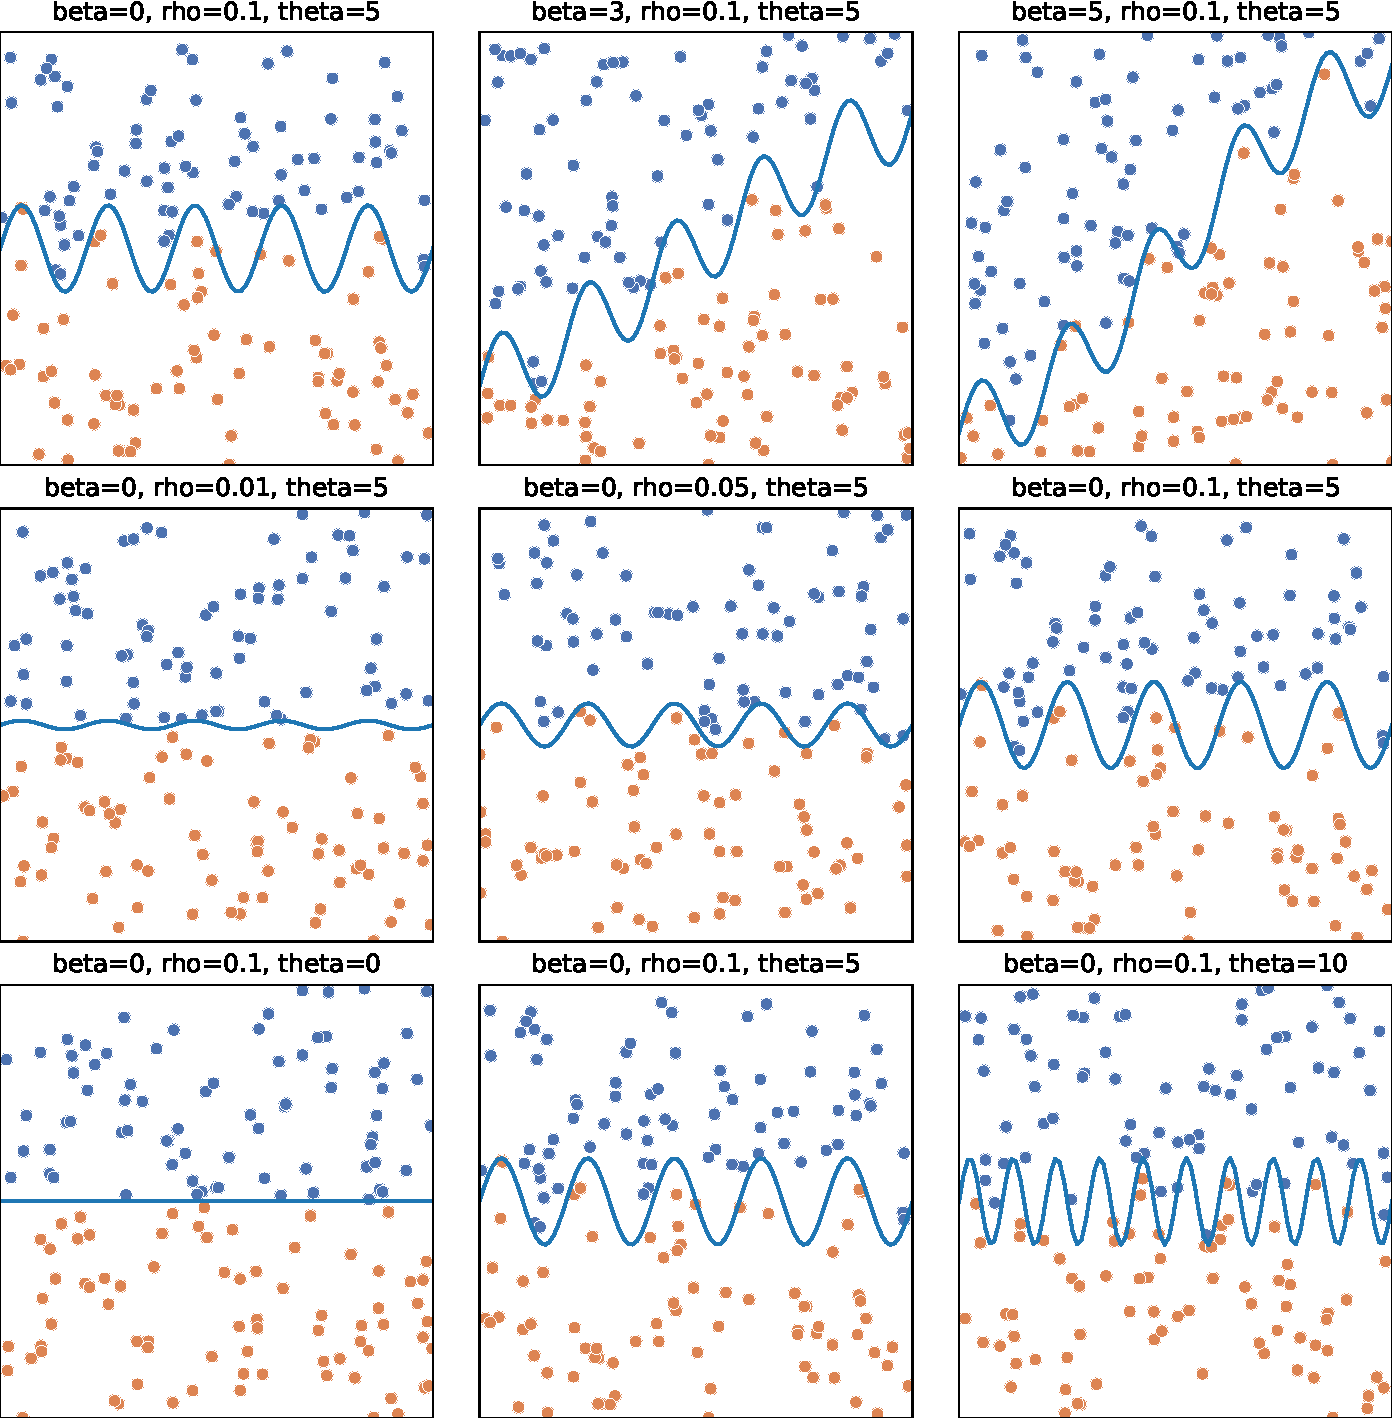
\includegraphics[width=.7\linewidth]{img/sinusoid_dataset_param_influence.pdf}
    \caption{Esempio di dataset generati con funzione sinusoidale. 
    $\beta$ controlla la pendenza, $\rho$ controlla l'ampiezza, $\theta$ la frequenza.}
    \label{fig:sinusoid_dataset}
\end{figure}
\begin{figure}
    \centering
    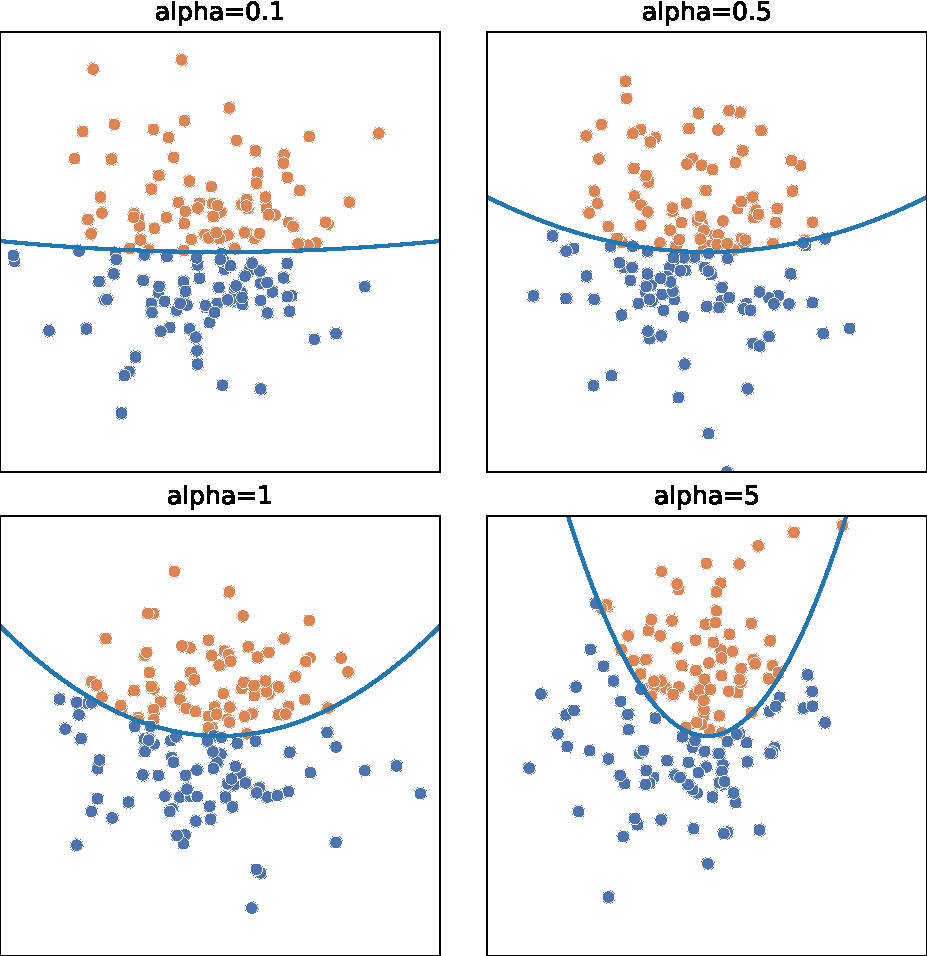
\includegraphics[width=.5\linewidth]{img/pacman_dataset_param_influence.pdf}
    \caption{Esempio di dataset etichettati con paraboloide. Il parametro $\alpha$ controlla l'ampiezza.}
    \label{fig:pacman_dataset}
\end{figure}
A prescindere dalla funzione di etichettatura utilizzata, la procedura di generazione del dataset è descritta nell'\Cref{alg:generazione_dataset_sintetici}.
Questa procedura richiede dei parametri aggiuntivi per regolare il bilanciamento tra le classi e la quantità di rumore:
\begin{itemize}
    \item Il parametro 
    \begin{equation*}
        p = \frac{\text{numero di elementi con etichetta positiva}}{\text{numero di elementi con etichetta negativa}}
    \end{equation*} 
    regola la proporzione tra esempi negativi ed esempi positivi.
    \item Il parametro $r$ indica la percentuale di elementi della classe positiva e altrettanti esempi della classe negativa da selezionare a caso per poi invertirne l'etichetta.
\end{itemize}
\begin{algorithm}
    \SetAlgoLined
    \KwData{
        $n>0 \in \mathrm{N}$ dimensione del dataset desiderata\\ 
        $p \in [0,1]$ per regolare il bilanciamento tra classi\\
        $r \in [0,1]$ per regolare la quantità di rumore\\
        \textit{test\_size} percentuale di dati da ritornare come \emph{test set}\\
        $s$ seme per le operazioni casuali\\
    }
    \KwResult{Dati $X$ ed etichette $y$ suddivisi in addestramento e test}
    Inizializza generatore casuale utilizzando il seme $s$\;
    $X_{pop} \gets$ seleziona a caso $10*n$ sample\;
    $y_{pop} \gets$ etichetta $X_{pop}$ con la funzione di etichettatura\;
    %
    $N_p \gets \lfloor\frac{n}{p + 1}\rfloor$\;
    $N_n \gets n - N_p$\;
    $X, y \gets$ seleziona a caso $N_p$ sample con etichetta positiva e $N_n$ sample con etichetta negativa da $X_{pop},y_{pop}$\;
    seleziona a caso $\lfloor r * N_p \rfloor$\ esempi della calsse positiva ed altrettanti elementi della classe negativa per cui invertire l'etichetta\;
    $X_{test}, y_{test} \gets$ seleziona \textit{test\_size} elementi (con rispettive etichette) a caso come test set\;
    $X_{train} \gets X \setminus X_{test}$\;
    $y_{train} \gets y \setminus y_{test}$\;
\caption{Procedura generica per la generazione di dataset sintetico.}
\label{alg:generazione_dataset_sintetici}
\end{algorithm}

% \subsubsection{Funzione sinusoidale}
% Fissando i parametri $\beta,\rho,\theta$, per un vettore $\Vec{x}=\{x_1,x_2\}$, l'etichetta $y$ è calcolata con la funzione
% \begin{equation}\label{eq:sinusoid_dataset_lf}
% lf(\Vec{x}) = \sign\left(\frac{1}{(1 + \exp(-\beta(x_1 - 0.5)) + \rho \sin(2\pi\theta x_1)} - x2\right).
% \end{equation}
% Questa funzione di etichettatura è utilizzata solo per dati in spazi con due dimensioni. La~\cref{fig:sinusoid_dataset} mostra alcuni esempi di dataset e funzioni di etichettatura al variare dei parametri.
% \begin{figure}
%     \centering
%     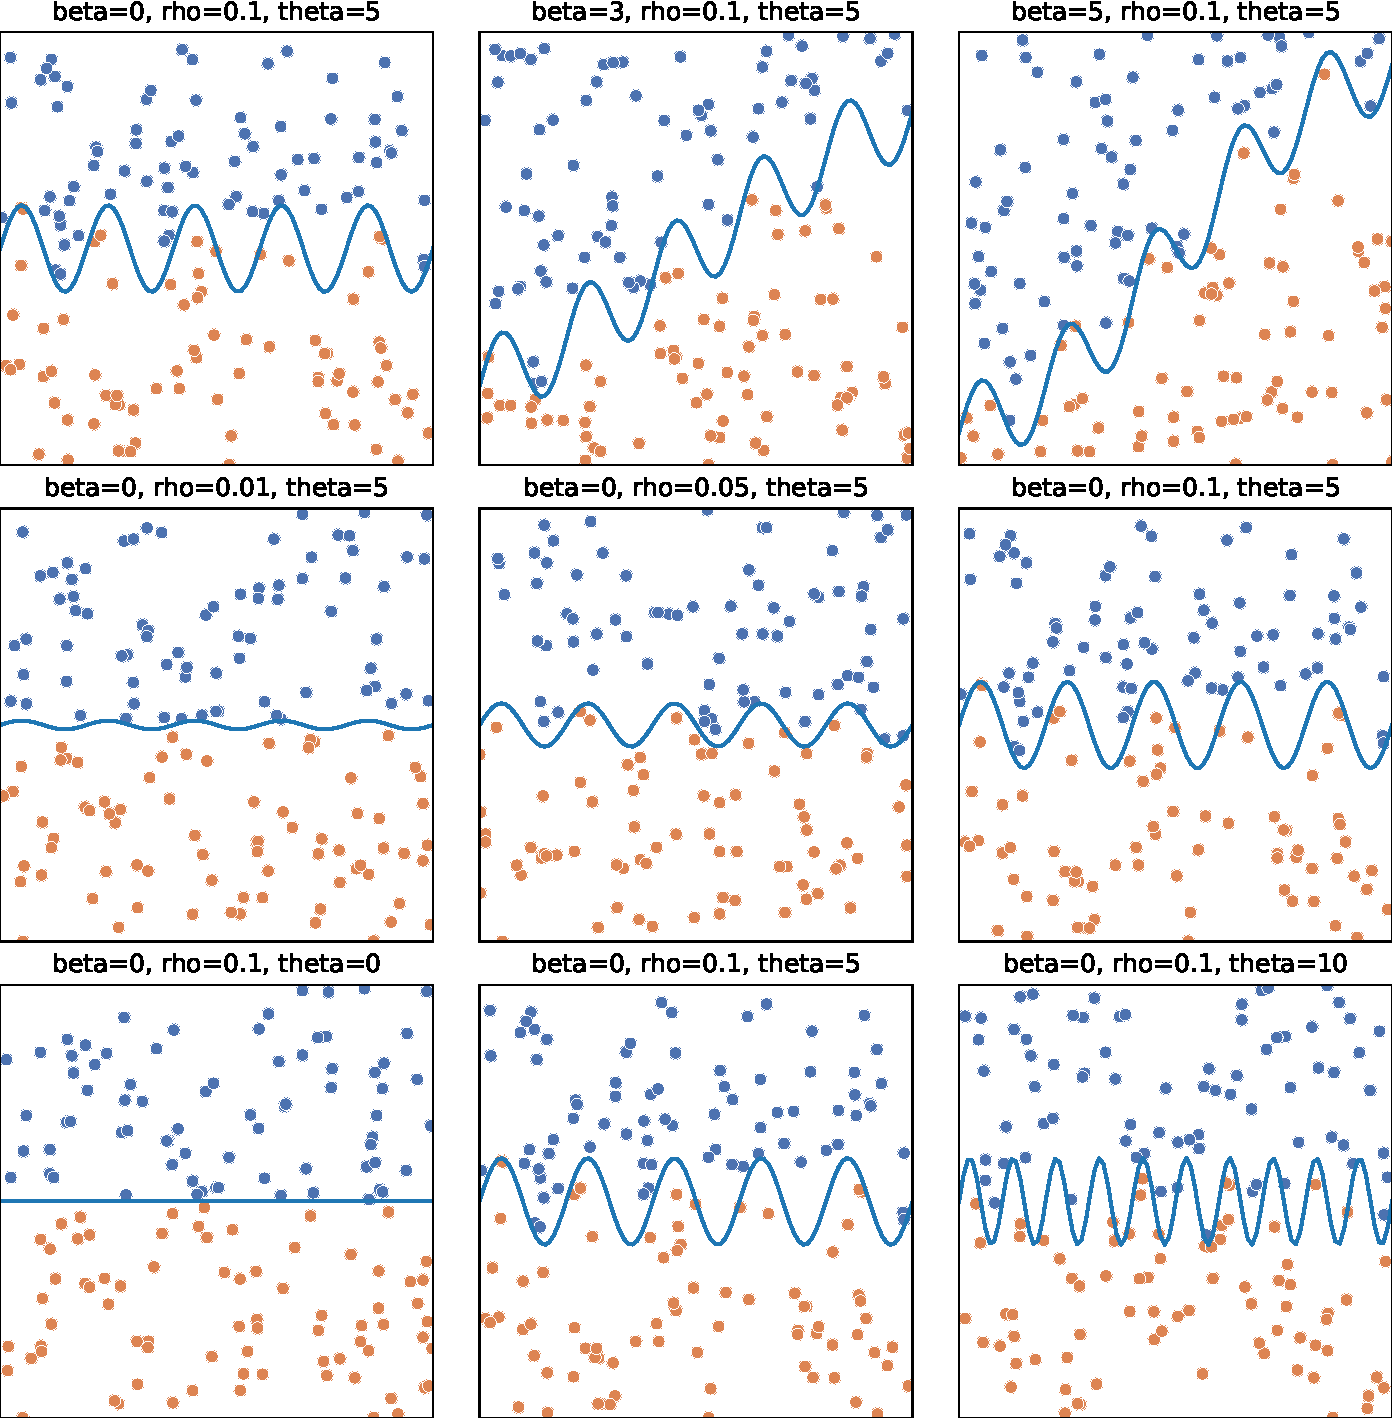
\includegraphics[width=1\linewidth]{img/sinusoid_dataset_param_influence.pdf}
%     \caption{Esempio di dataset generati con funzione sinusoidale. 
%     $\beta$ controlla la pendenza, $\rho$ controlla l'ampiezza, $\theta$ la frequenza.}
%     \label{fig:sinusoid_dataset}
% \end{figure}
% \subsubsection{Funzione paraboloide}
% Fissati i parametri $\alpha, x_\text{shift}, y_\text{shift}$, per un vettore $\Vec{x}=\{x_1, \dots, x_n\} \in \mathrm{R}^n$, l'etichetta $y$ è calcolata con la funzione
% \begin{equation}\label{eq:pacman_dataset_lf}
% lf(\Vec{x})= x_n - \sum_{i=1}^{n-1}\alpha(x_i - x_\text{shift})^2 - y_\text{shift}.
% \end{equation}
% Il parametro $\alpha$ controlla l'ampiezza del paraboloide, mentre $x_\text{shift}$ e $y_\text{shift}$ traslano il vertice del paraboloide.
% La~\Cref{fig:pacman_dataset} mostra alcuni esempi di dataset e funzioni di etichettatura al variare dei parametri.
% \begin{figure}
%     \centering
%     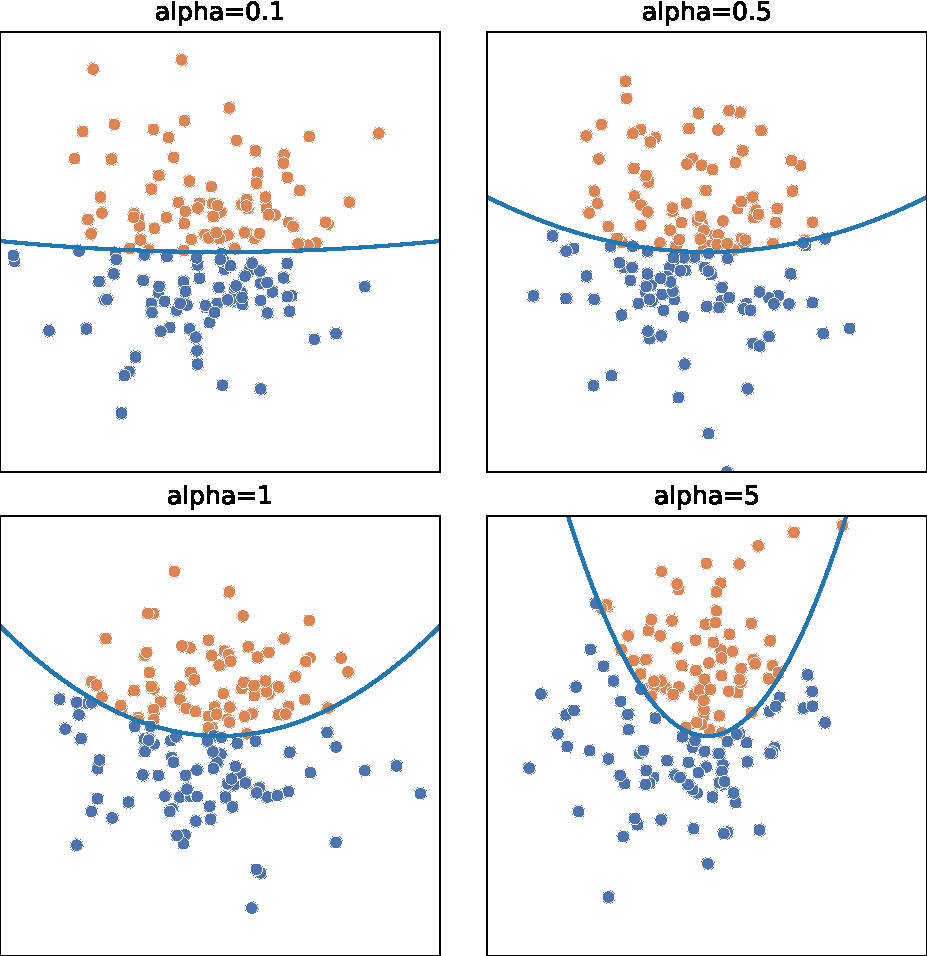
\includegraphics[width=1\linewidth]{img/pacman_dataset_param_influence.pdf}
%     \caption{Esempio di dataset etichettati con paraboloide. Il parametro $\alpha$ controlla l'ampiezza.}
%     \label{fig:pacman_dataset}
% \end{figure}
I parametri per le funzioni di etichettatura utilizzati per la generazione dei dataset sono scelti in modo da avere vari livelli di ``difficoltà'' di classificazione, misurata con le metriche esposte in~\Cref{sec:metriche_dataset}.
La difficoltà può essere gradualmente aumentata per esempio stringendo progressivamente il paraboloide o aumentando la frequenza o l'ampiezza della funzione sinusoidale.

La procedura nell'~\Cref{alg:generazione_dataset_sintetici} utilizza delle estrazioni casuali in diversi punti:
\begin{itemize}
    \item per selezionare la popolazione iniziale;
    \item per estrarre i dati di test;
    \item eventualmente nella procedura di introduzione del rumore, per selezionare degli esempi a cui invertire l'etichetta.
\end{itemize}
Per rendere la generazione ripetibile, l'~\Cref{alg:generazione_dataset_sintetici} richiede un parametro seme.


\subsection{Dataset di terze parti}
I dataset di terze parti utilizzati per alcuni esperimenti provengono dalla pagina web della libreria LibSVM\footnote{\url{https://www.csie.ntu.edu.tw/~cjlin/libsvmtools/datasets/binary.html}}.
Sono dataset utilizzati in letteratura ma pre-elaborati (scalando e normalizzando gli attributi) e resi disponibili in formato LibSVM~\cite{libsvm}.
Si riportano in~\Cref{tab:uci_datasets} le caratteristiche dei dataset utilizzati.
\begin{table}
    \centering
    \begin{tabular}{cccc}
        \toprule
        Nome & Num. dati train & Num. dati test & Num. feature\\
        \midrule
        svmguide1 &  3,089 & 4,000 & 4 \\
        a1a & 1,605	& 30,956 & 123\\
        gisette & 6000 & 1000 & 5000 \\
        \bottomrule
    \end{tabular}
    \caption{Caratteristiche dataset di terze parti.}
    \label{tab:uci_datasets}
\end{table}


\section{Impostazione esperimenti}
In generale ogni esperimento effettuato sul metodo proposto consiste nel selezionare il miglior modello per un dato dataset al variare di valori di \emph{budget}.
Con miglior modello, nel resto di questo capitolo, si intende il miglior modello selezionato da \emph{5-fold cross validation grid search} valutando la metrica accuratezza. 

Per cercare di ridurre il carico computazionale, gli esperimenti effettuati utilizzando il modello \emph{budgeted SVC} utilizzano una matrice \emph{kernel} pre-calcolata; le implementazioni di altri metodi presenti in letteratura utilizzati come confronto, invece, calcolano i valori di \emph{kernel} durante l'addestramento.

Tutti gli esperimenti sono stati eseguiti su un server con CPU Intel(R) Xeon(R) W-1250P CPU @ 4.10GHz e con 31GB di ram. Il linguaggio di programmazione utilizzato è Python 3.10.10 ed è stato utilizzato il risolutore Gurobi 10.0.1~\cite{gurobi}.

\section{Esperimenti su dataset sintetici 2D}\label{sec:exp:synth_2d}
Si riportano in questo paragrafo gli esperimenti effettuati sui dataset sintetici generati con le configurazioni di parametri riportate nelle~\Cref{tab:parametri_ds_sin,tab:parametri_ds_pacman}.
Per questi dataset, a prescindere dal resto dei parametri, sono stati generati 1000 punti totali, di cui 700 per l'addestramento e 300 per la fase di \emph{test}. Il seme utilizzato ha valore $42$.
\begin{table}
    \centering
    \begin{tabular}{ccc}
        \toprule
        $\beta$ & $\rho$ & $\theta$\\
        \midrule
        \multirow{5}{*}{0}  & 0.01  & \multirow{5}{*}{20} \\        
                            & 0.025 &     \\        
                            & 0.05  &     \\        
                            & 0.075 &     \\        
                            & 0.1   &     \\
        \hline
        95                  & 0.2   & 10    \\   
        \hline
        \multirow{4}{*}{0}  & \multirow{4}{*}{0.1}  & 1     \\    
                            &                       & 2     \\    
                            &                       & 5     \\    
                            &                       & 1     \\    
        \bottomrule
    \end{tabular}
    \caption{Configurazioni di parametri utilizzati per generare dataset bidimensionali con la funzione sinusoidale in~\Cref{eq:sinusoid_dataset_lf}.}
    \label{tab:parametri_ds_sin}
\end{table}
\begin{table}
    \centering
    \begin{tabular}{ccc}
        \toprule
        $\alpha$ & $x_\text{shift}$ & $y_\text{shift}$ \\
        \midrule
        1   & \multirow{5}{*}{0.5} & \multirow{5}{*}{0.5} \\
        2.5 &\\
        5   &\\
        7.5 &\\
        10  &\\
        \bottomrule
    \end{tabular}
    \caption{Configurazioni di parametri utilizzati per generare dataset bidimensionali con la funzione paraboloide in~\Cref{eq:pacman_dataset_lf}.}
    \label{tab:parametri_ds_pacman}
\end{table}

\subsubsection{Budget in funzione del modello classico}
Una parte consistente degli esperimenti è stata eseguita seguendo la procedura descritta nell'~\Cref{alg:esperimenti_1}.
Per prima cosa si addestra un modello SVM tradizionale senza nessun vincolo sul numero di vettori di supporto.
In seguito si addestrano una serie di modelli con un \emph{budget} pari ad una frazione dei vettori di supporto del modello classico addestrato al passo precedente.
\begin{algorithm}
    \SetAlgoLined
    \KwData{$ds$ dataset}
    %\KwResult{}
    $FM \gets$ seleziona il miglior modello senza imporre nessun vincolo di budget\;
    $FB \gets$ numero di vettori di supporto del modello $FM$\;
    salva parametri e dettagli di $FM$\;
    \For{$p\gets0.3$ \KwTo $0.9$ \KwBy $0.1$}{
        $B\gets p*FB$\;
        $M \gets$ seleziona il miglior modello con $\text{budget}=B$\;
        salva parametri e dettagli di $M$\;
    }
\caption{Pseudocodice esperimenti sullo stesso dataset ma con budget in funzione del numero di vettori di supporto del modello classico.}
\label{alg:esperimenti_1}
\end{algorithm}
L'obiettivo di questo tipo di esperimenti è quello di analizzare l'accuratezza sui dati di \emph{test} al diminuire del \emph{budget}.
Il \emph{budget} è espresso come $B=p*FM$, dove $FM$ è il numero di vettori di supporto di un modello addestrato senza vincolo sul \emph{budget} e dove
\begin{equation*}
    p\in\{0.3, 0.4, 0.5, 0.6, 0.7, 0.8, 0.9\}.
\end{equation*}

Con questi esperimenti è possibile ottenere delle indicazioni su quanto sia possibile ridurre il budget senza penalizzare troppo le \emph{performance}, limitatamente ai dataset considerati e in rapporto alla controparte senza vincolo sul budget.

Per avere un risultato più robusto, mitigando un eventuale \emph{bias} introdotto dalla selezione casuale di elementi del dataset, si è deciso di generare 3 dataset con gli stessi parametri utilizzando però un seme diverso per la selezione casuale.
In generale quindi la procedura completa è descritta nell'~\Cref{alg:esperimenti_2}.
\begin{algorithm}
    \SetAlgoLined
    \For{params \KwIn \text{parametri dataset}}{
        \For{$s \gets \text{estrai nuovo seme}$}{
            $ds\gets$ genera dataset con l'~\Cref{alg:generazione_dataset_sintetici} usando $params$ e $s$\;
            esegui l'~\Cref{alg:esperimenti_1} su $ds$\;           
        }
    }
\caption{Pseudocodice esperimenti con ripetizione della generazione dei dataset}
\label{alg:esperimenti_2}
\end{algorithm}

Ogni modello è selezionato con \emph{5-fold cross validation grid search} utilizzando i parametri descritti in~\Cref{tab:gridsearch_2d}.
\begin{table}
    \centering
    \begin{tabular}{cccc}
        \toprule
        $C$ & \emph{Kernel} & $\gamma$ & d \\
        \midrule
        \multirow{3}{*}{[0.01, 0.1, 1, 10]} & Gaussiano   & [0.0001, 0.001, 0.01, 0.1, 1, 10]   & /\\
                                            \cline{2-4}
                                            & Polinomiale   & / & [2, 5, 10] \\
                                            \cline{2-4}
                                            & Lineare       & / & / \\
        \bottomrule
    \end{tabular}
    \caption{Parametri \emph{grid search} per gli esperimenti su dataset bidimensionali.}
    \label{tab:gridsearch_2d}
\end{table}

Nelle~\Cref{fig:risultati_2d_1,fig:risultati_2d_2} si riportano dei grafici per analizzare l'accuratezza ottenuta sui dati di \emph{test} sia in termini assoluti che in rapporto con l'accuratezza del modello senza vincolo sul \emph{budget}.
Per un modello, si definisce \emph{score ratio} la quantità
\begin{equation*}
    \text{score ratio} = \frac{\text{accuratezza su dati di test del modello con vincolo sul budget}}{\text{accuratezza su dati di test del modello senza budget}}.
\end{equation*}
\begin{figure}
    \begin{subfigure}{.5\textwidth}
        \centering
        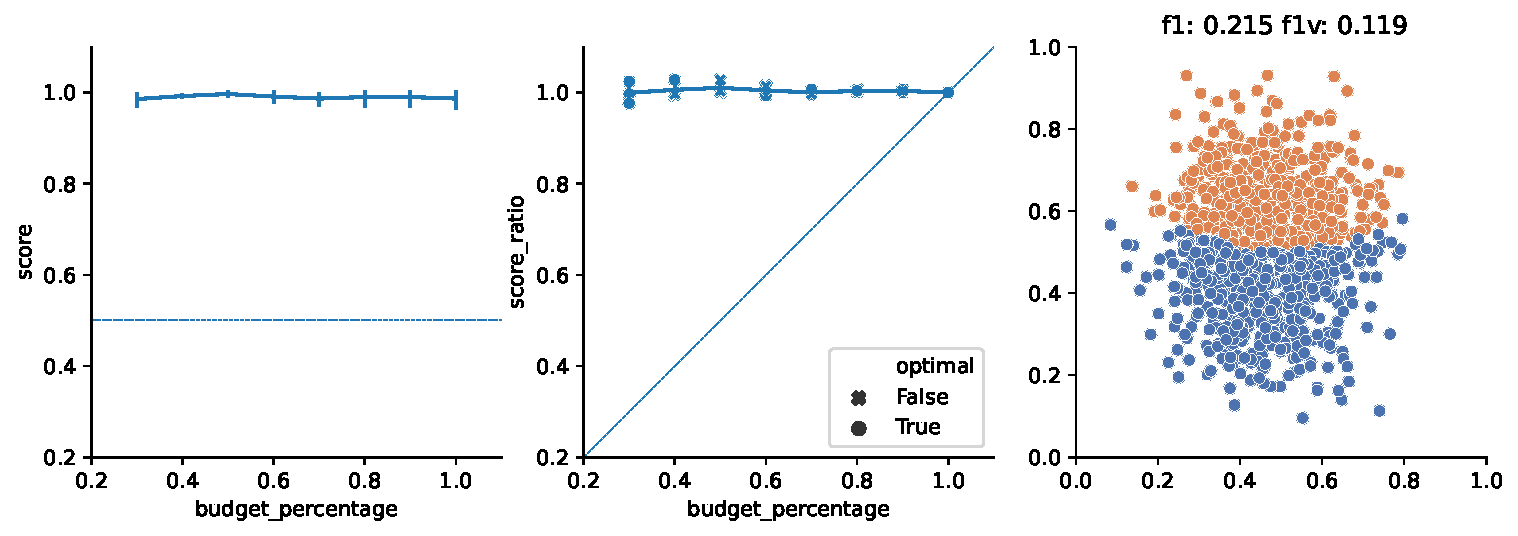
\includegraphics[width=\textwidth]{img/2d/1.pdf}
    \end{subfigure}%
    \begin{subfigure}{.5\textwidth}
        \centering
        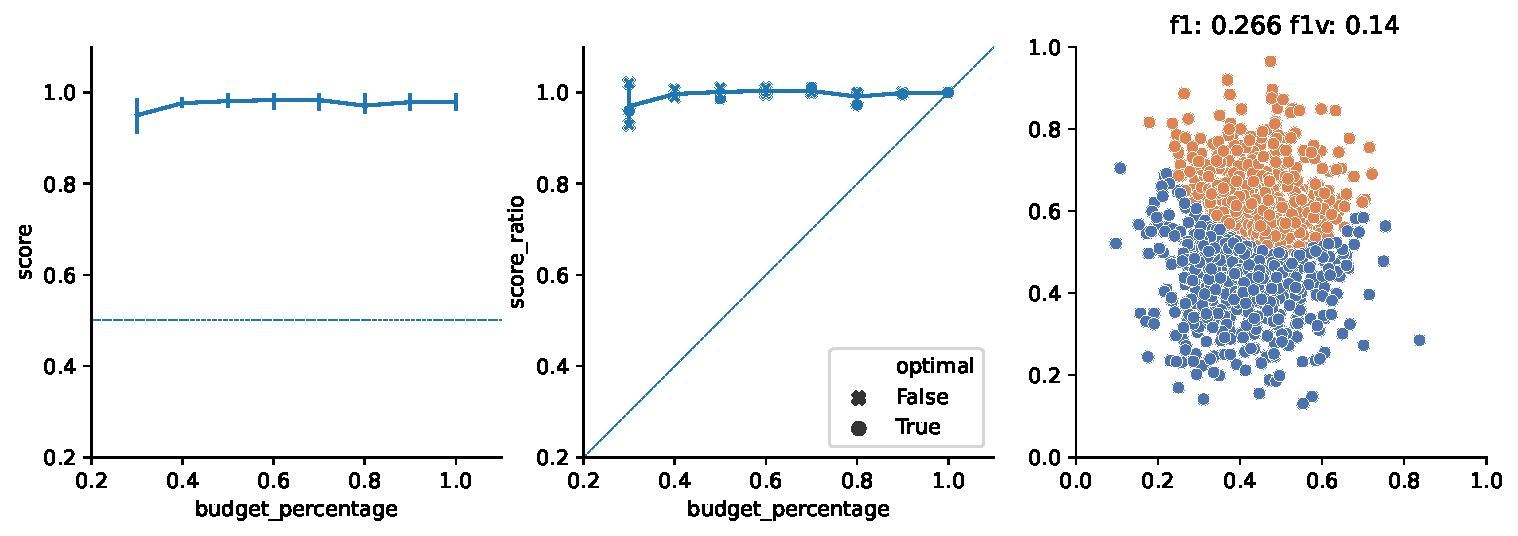
\includegraphics[width=\textwidth]{img/2d/2.pdf}
    \end{subfigure}%
    %
    \hfill
    %
    \begin{subfigure}{.5\textwidth}
        \centering
        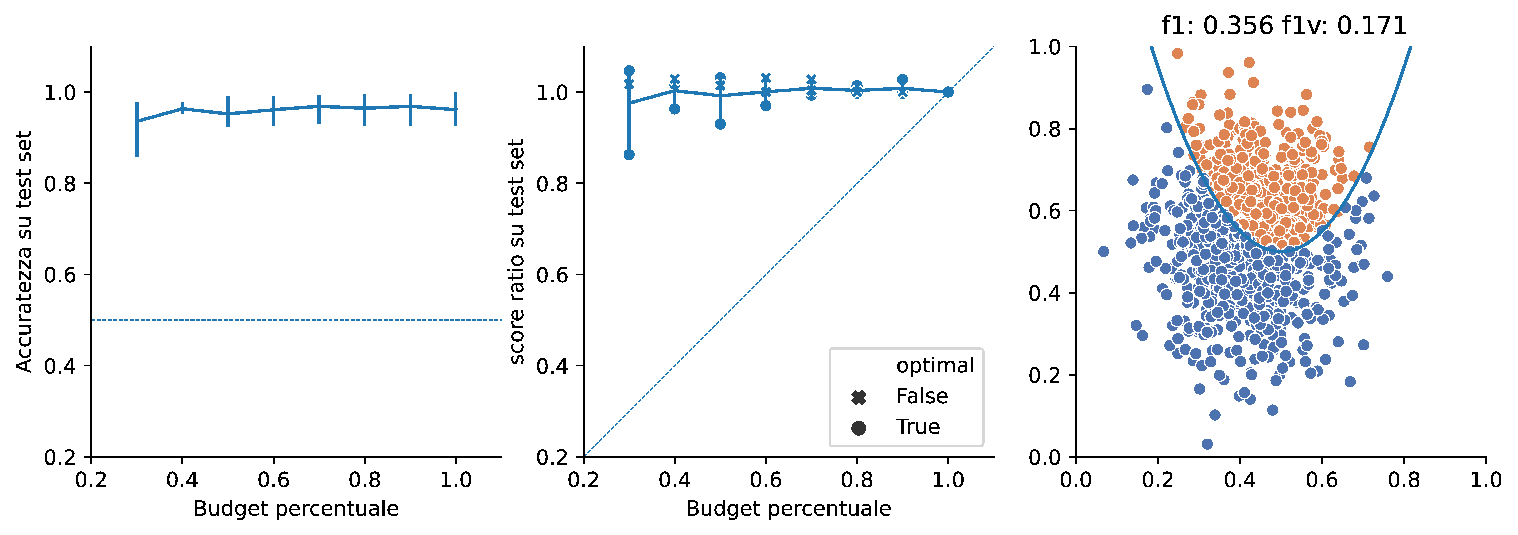
\includegraphics[width=\textwidth]{img/2d/3.pdf}
    \end{subfigure}%
    \begin{subfigure}{.5\textwidth}
        \centering
        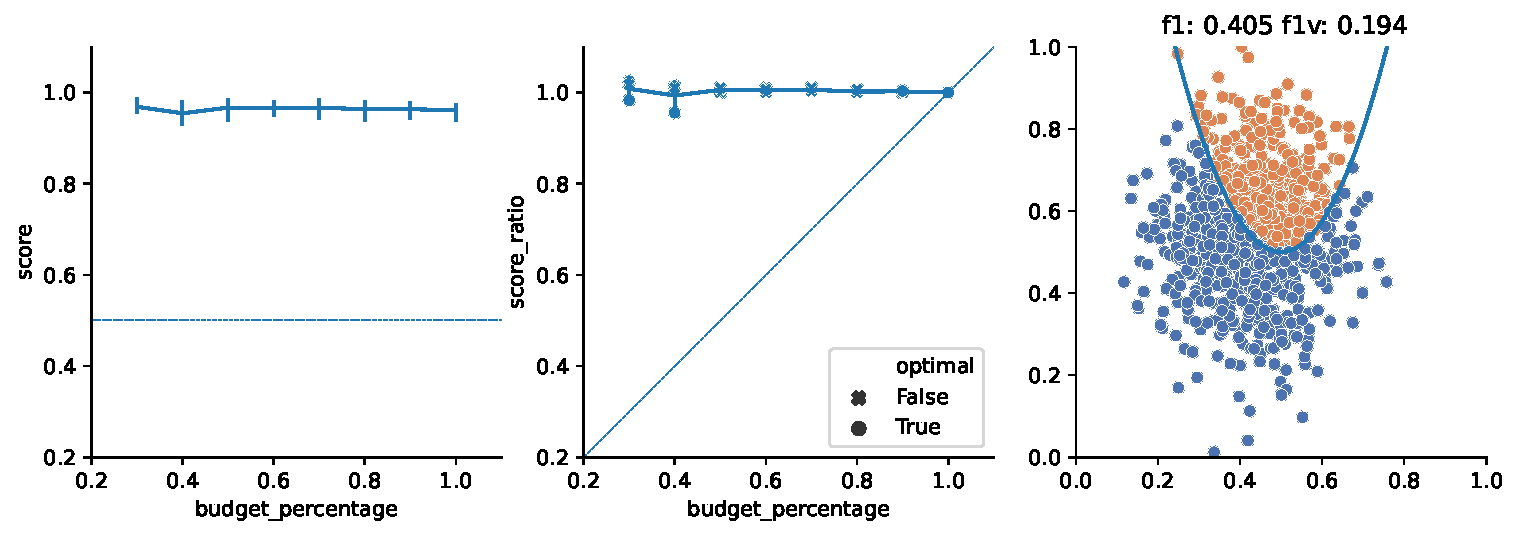
\includegraphics[width=\textwidth]{img/2d/4.pdf}
    \end{subfigure}%
    %
    \hfill
    %
    \begin{subfigure}{.5\textwidth}
        \centering
        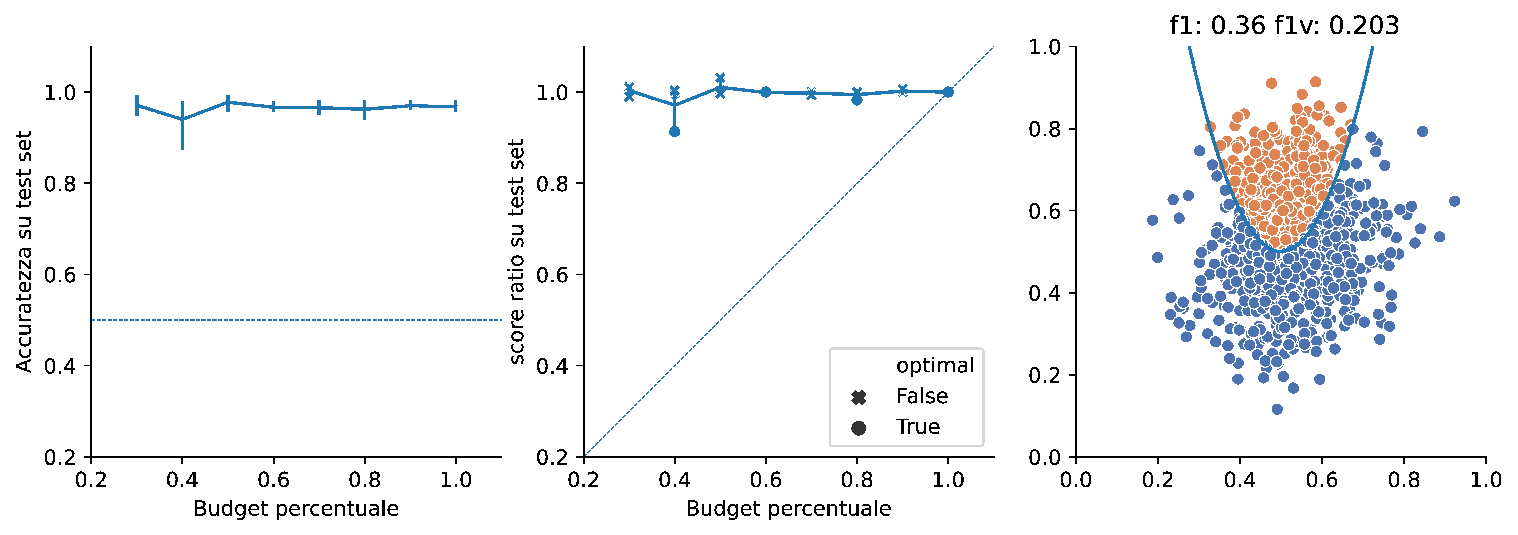
\includegraphics[width=\textwidth]{img/2d/5.pdf}
    \end{subfigure}%
    \begin{subfigure}{.5\textwidth}
        \centering
        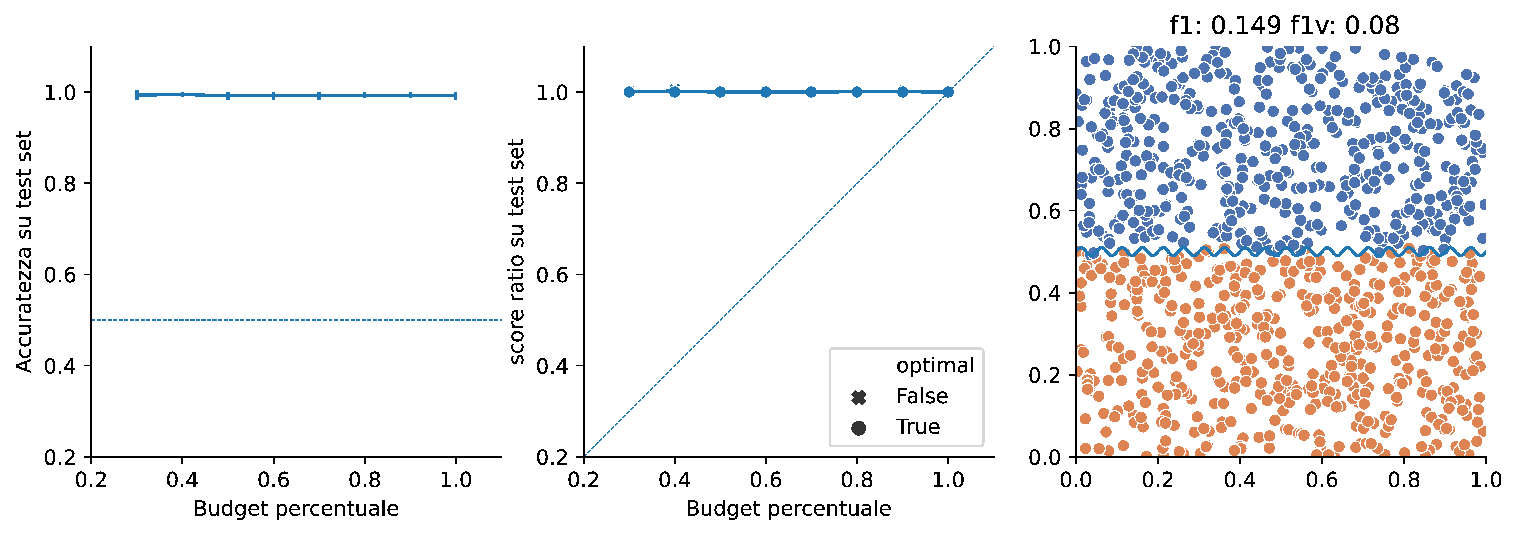
\includegraphics[width=\textwidth]{img/2d/6.pdf}
    \end{subfigure}%
    %
    \hfill
    %
    \begin{subfigure}{.5\textwidth}
        \centering
        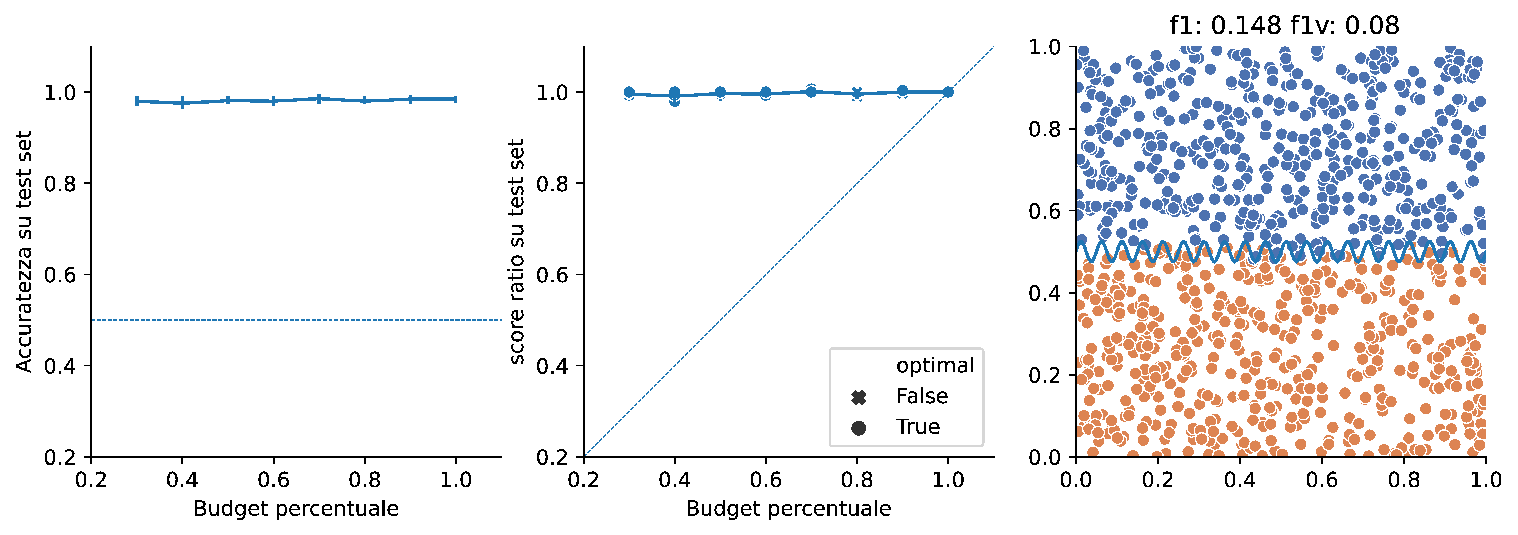
\includegraphics[width=\textwidth]{img/2d/7.pdf}
    \end{subfigure}%
    \begin{subfigure}{.5\textwidth}
        \centering
        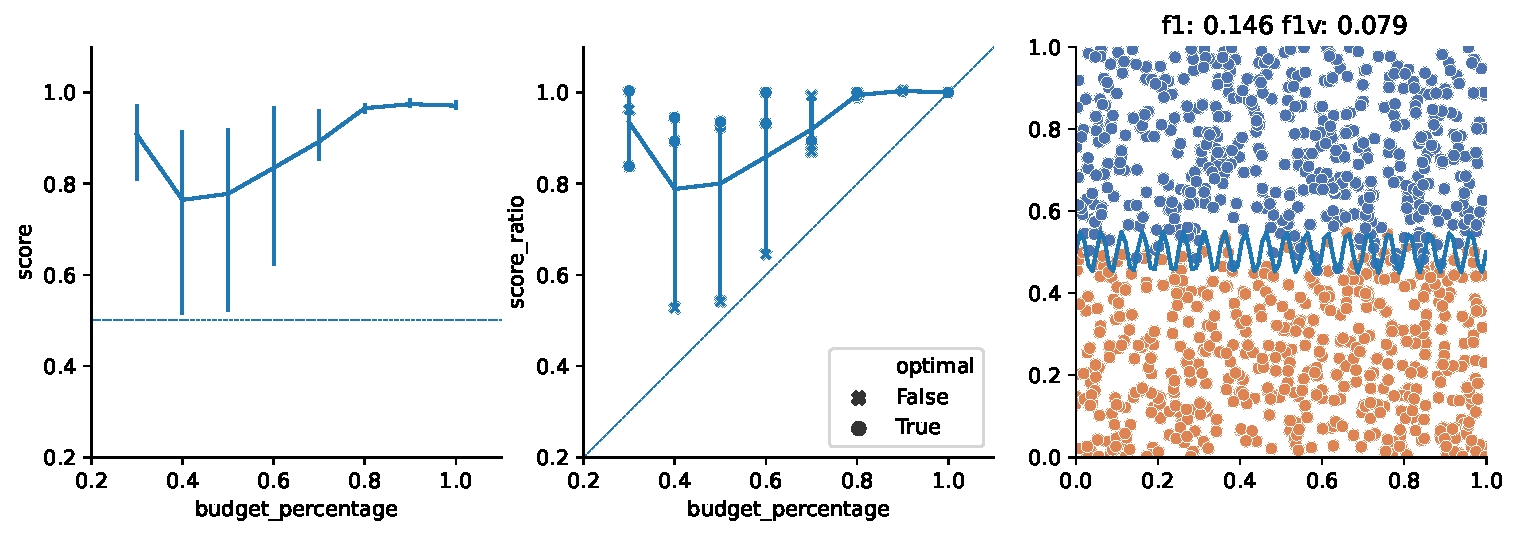
\includegraphics[width=\textwidth]{img/2d/8.pdf}
    \end{subfigure}%

\caption{Risultati degli esperimenti su dataset sintetici dove il budget è espresso in funzione di un modello classico. Ognuno dei grafici a sinistra indica l'andamento dell'accuratezza sui dati di \emph{test} al variare del \emph{budget}; ognuno dei grafici al centro indica l'accuratezza sui dati di \emph{test} in rapporto all'accuratezza del modello senza vincolo sul \emph{budget} (\emph{optimal} si riferisce allo stato del solver gurobi); ognuno dei grafici a destra rappresenta il dataset utilizzato con le rispettive misure di ``difficoltà''.}
\label{fig:risultati_2d_1}
\end{figure}
\begin{figure}
\begin{subfigure}{.5\textwidth}
        \centering
        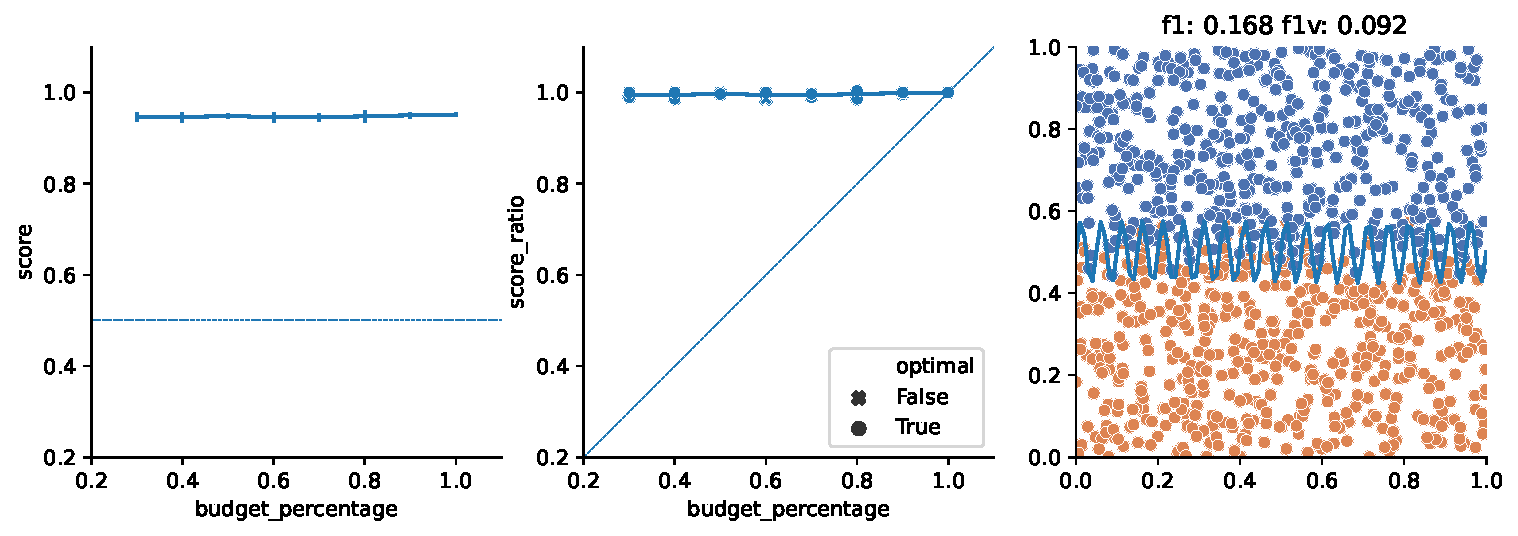
\includegraphics[width=\textwidth]{img/2d/9.pdf}
    \end{subfigure}%
    \begin{subfigure}{.5\textwidth}
        \centering
        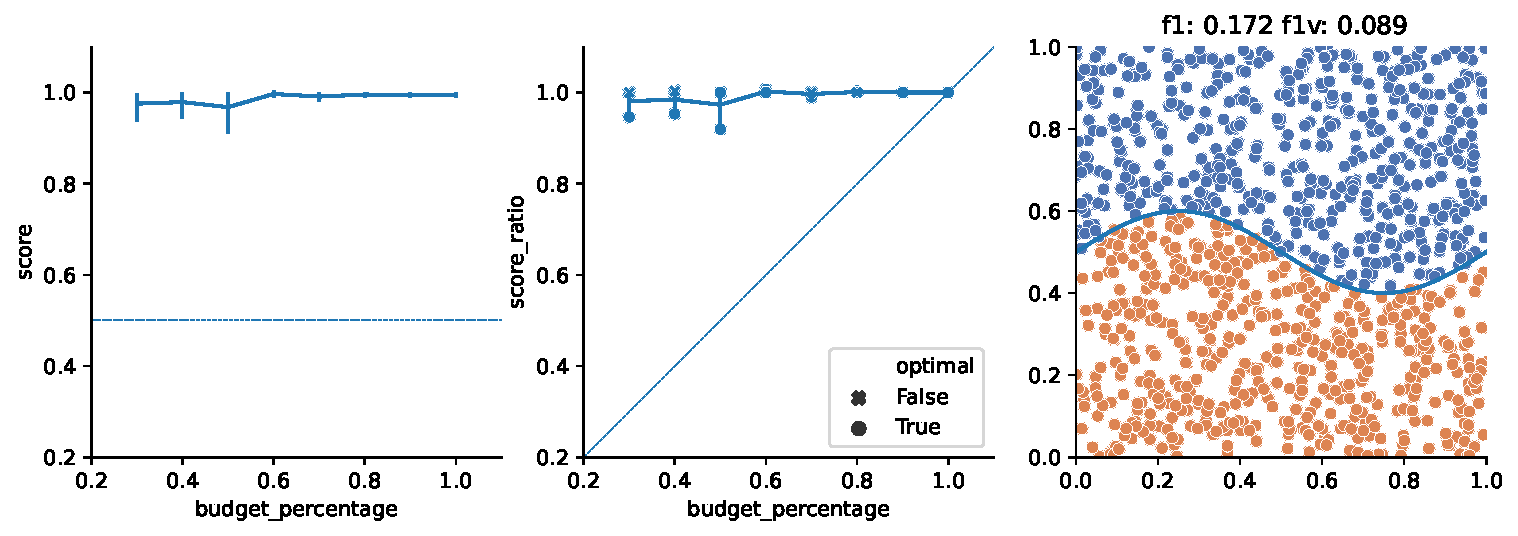
\includegraphics[width=\textwidth]{img/2d/10.pdf}
    \end{subfigure}%
     %
    \hfill
    %
     \begin{subfigure}{.5\textwidth}
        \centering
        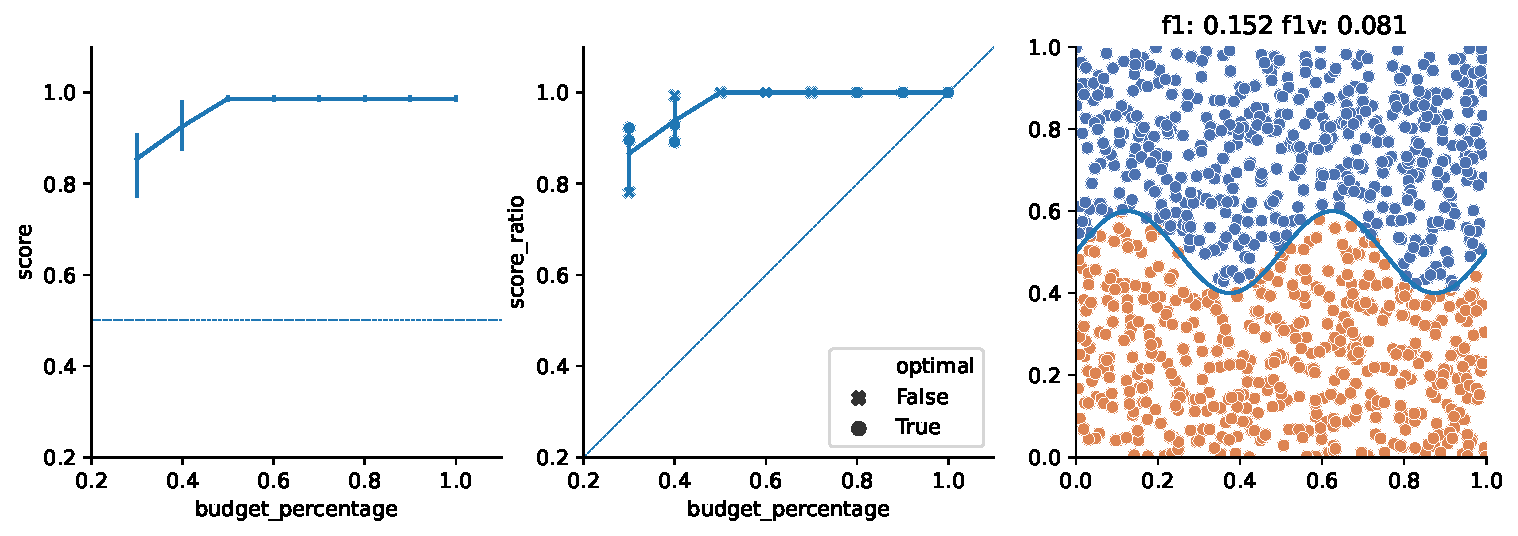
\includegraphics[width=\textwidth]{img/2d/11.pdf}
    \end{subfigure}%
    \begin{subfigure}{.5\textwidth}
        \centering
        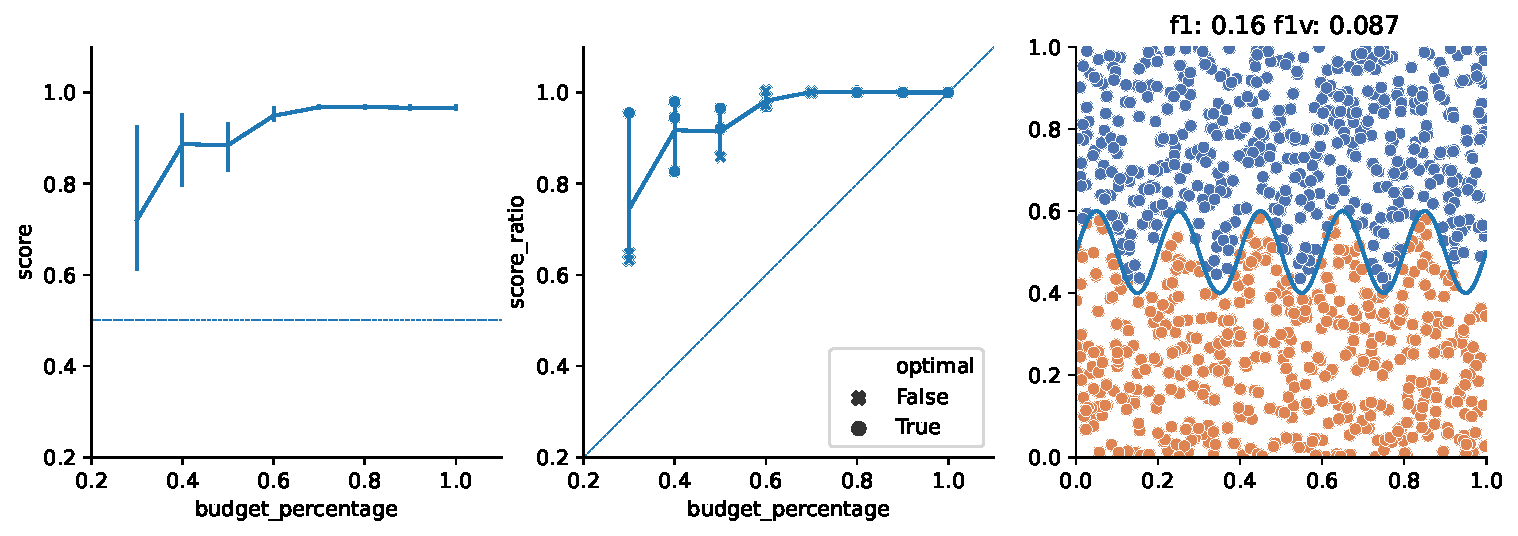
\includegraphics[width=\textwidth]{img/2d/12.pdf}
    \end{subfigure}%
     %
    \hfill
    %
    \begin{subfigure}{.5\textwidth}
        \centering
        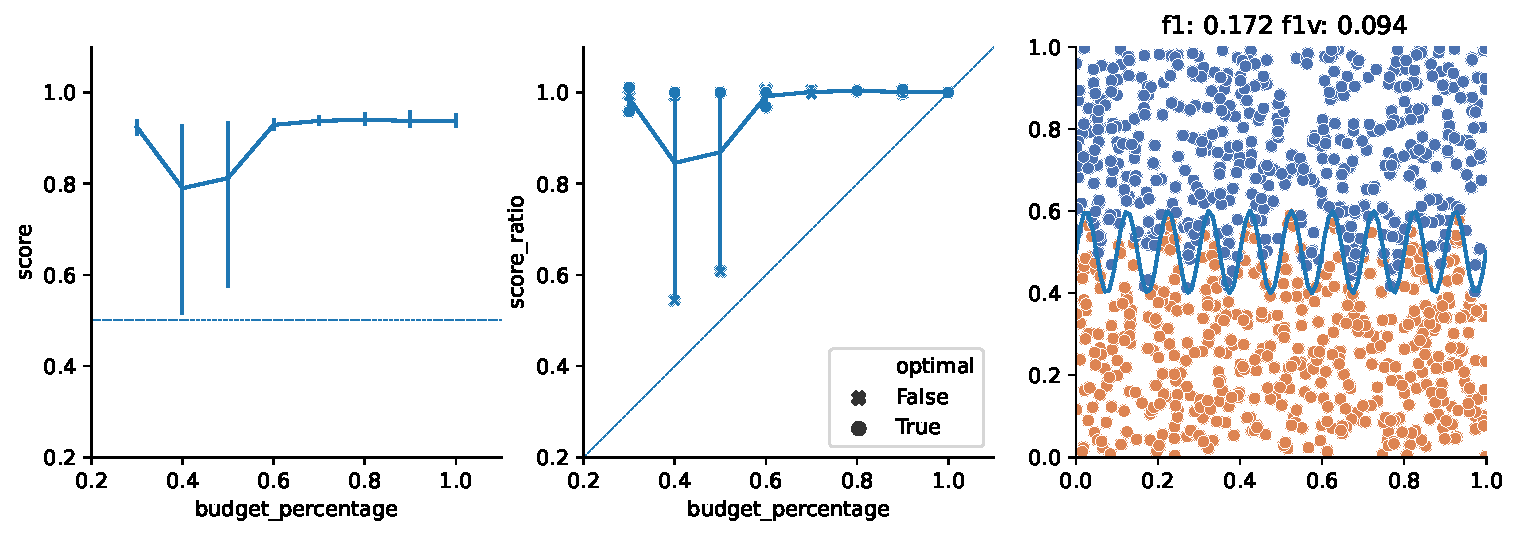
\includegraphics[width=\textwidth]{img/2d/13.pdf}
    \end{subfigure}%
    \begin{subfigure}{.5\textwidth}
        \centering
        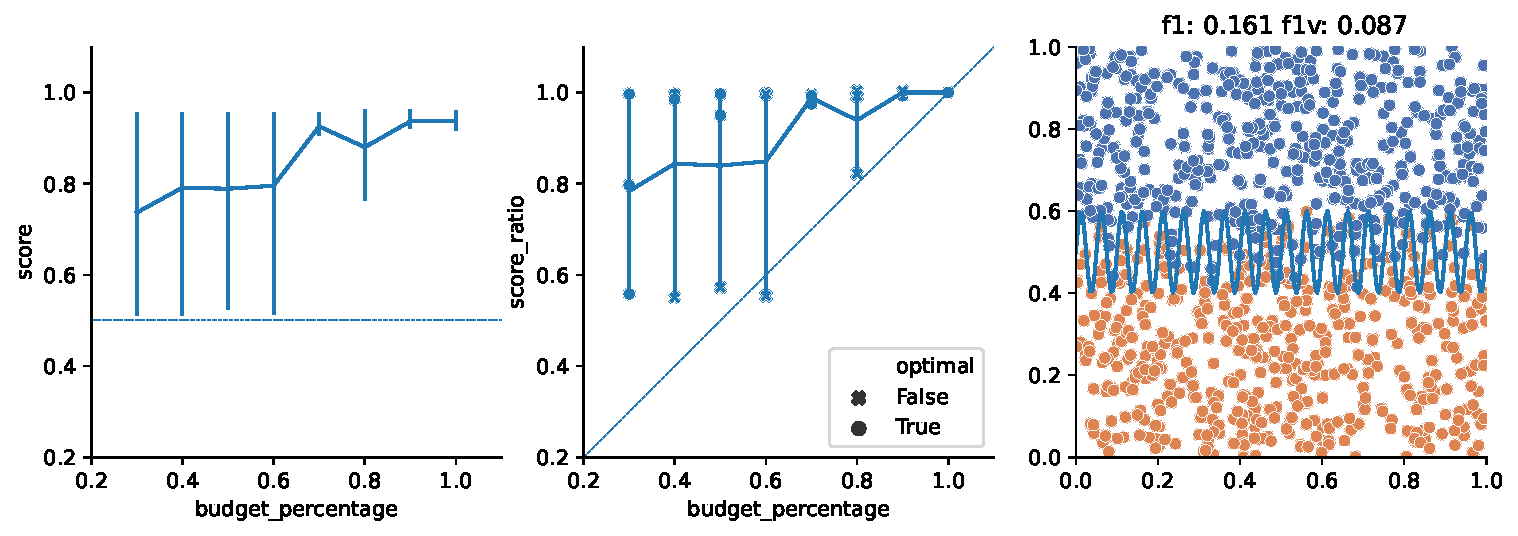
\includegraphics[width=\textwidth]{img/2d/14.pdf}
    \end{subfigure}%
     %
    \hfill
    %
    \begin{subfigure}{.5\textwidth}
        \centering
        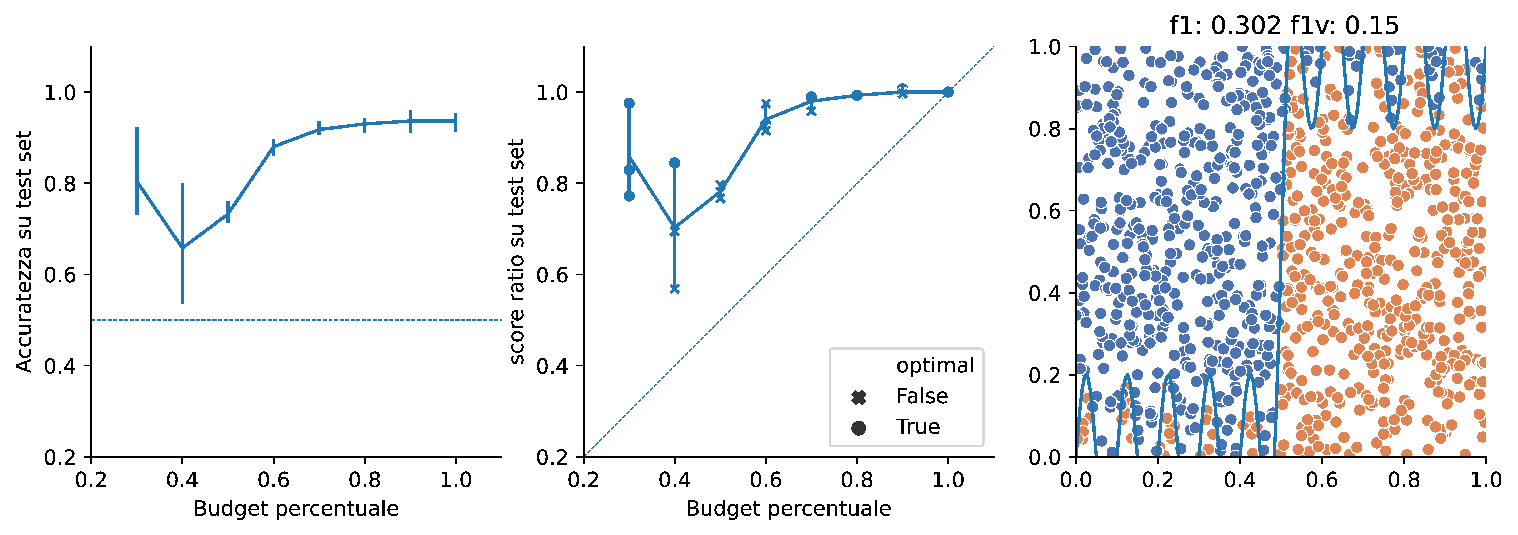
\includegraphics[width=\textwidth]{img/2d/15.pdf}
    \end{subfigure}%
    \caption{Risultati degli esperimenti su dataset sintetici dove il budget è espresso in funzione di un modello classico. Ognuno dei grafici a sinistra indica l'andamento dell'accuratezza sui dati di \emph{test} al variare del \emph{budget}; ognuno dei grafici al centro indica l'accuratezza sui dati di \emph{test} in rapporto all'accuratezza del modello senza vincolo sul \emph{budget} (\emph{optimal} si riferisce allo stato del solver gurobi); ognuno dei grafici a destra rappresenta il dataset utilizzato con le rispettive misure di ``difficoltà''.}
\label{fig:risultati_2d_2}
\end{figure}

Dai risultati ottenuti è possibile notare come per dataset ``semplici'', o con una funzione di etichettatura complessa ma ben approssimabile da una superficie lineare, il metodo proposto risulta efficace, portando ad una riduzione significativa del numero di vettori di supporto senza pagare troppo in termini di accuratezza.
In altri casi, invece, con dataset non necessariamente più difficili secondo le metriche F1 e F1v, le \emph{performance} peggiorano significativamente in relazione alla riduzione di vettori di supporto. In questi casi si nota anche un'alta variabilità nei risultati su dataset generati con stessi parametri ma con seme diverso.
% magari full_budget partiva già con "pochi" sv e ridurli porta ad accuracy molto più basse... ma non so

Si può anche notare come in alcuni casi il numero di vettori di supporto di un modello tradizionale senza vincolo sia molto alto in confronto alla dimensione del dataset.
**tabella che riporta il numero di vettori di supporto dei modelli full\_budget (?)**

\subsubsection{Budget in funzione della dimensione del dataset}
Un secondo approccio per eseguire gli esperimenti consiste nell'esprimere il budget in funzione della dimensione del dataset invece che in funzione di un modello senza vincolo sul budget.
Utilizzando gli stessi dataset sintetici degli esperimenti precedenti, si esprime il budget come $B=pm$, dove $m$ è il numero di elementi nel dataset e dove
\begin{equation*}
    p\in\{0.01, 0.025, 0.05, 0.075, 0.1, 0.125, 0.15, 0.175, 0.2\}.
\end{equation*}
Così facendo possiamo verificare quanto stringente possa essere il \emph{budget} imposto, anche utilizzando percentuali molto basse ($1\%$).
Per questi esperimenti i dataset sono stati generati una sola volta con un solo seme per ogni configurazione di parametri.
Nelle~\Cref{fig:2d_v2_1,fig:2d_v2_2} si riporta l'andamento dell'accuratezza sui dati di \emph{test} al variare del \emph{budget} per ogni dataset.
\begin{figure}
    \begin{subfigure}{.5\textwidth}
        \centering
        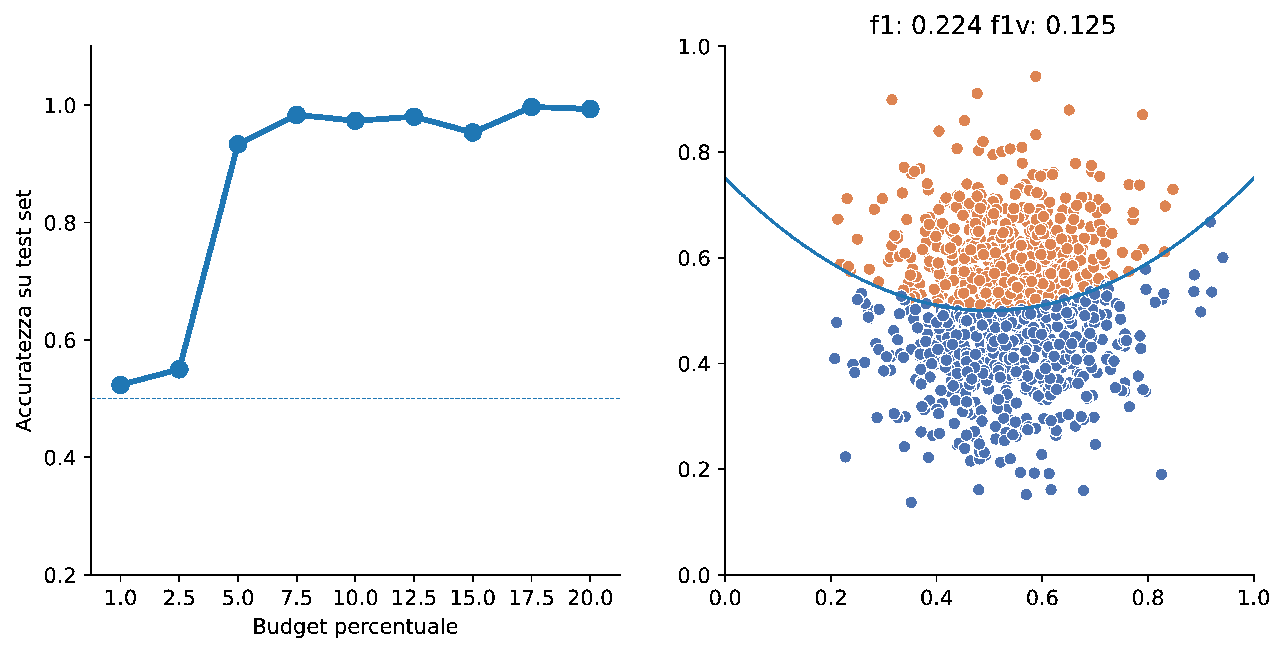
\includegraphics[width=\textwidth]{img/2d_v2/1.pdf}
    \end{subfigure}%
    \begin{subfigure}{.5\textwidth}
        \centering
        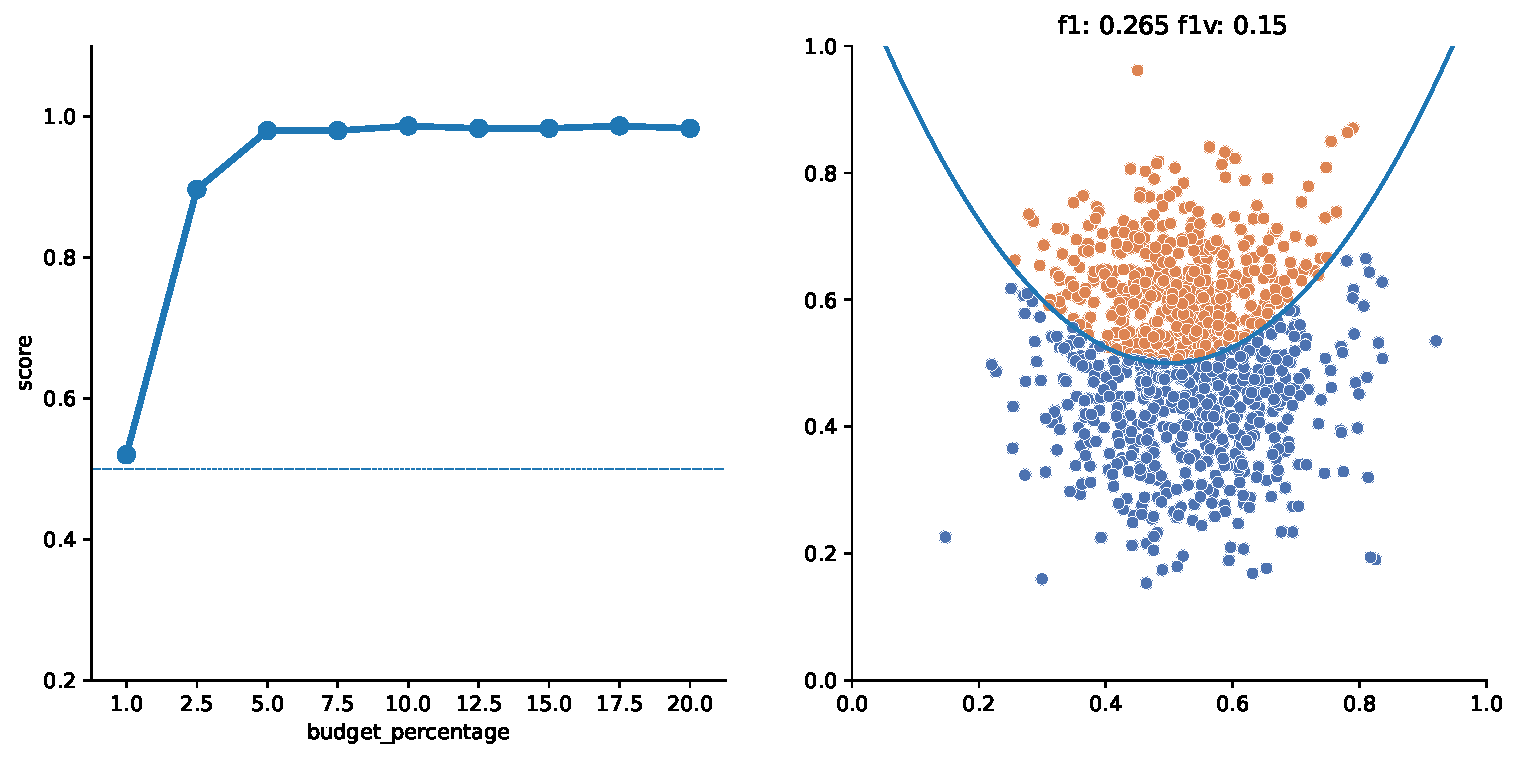
\includegraphics[width=\textwidth]{img/2d_v2/2.pdf}
    \end{subfigure}
    %
    \hfill
    %
    \begin{subfigure}{.5\textwidth}
        \centering
        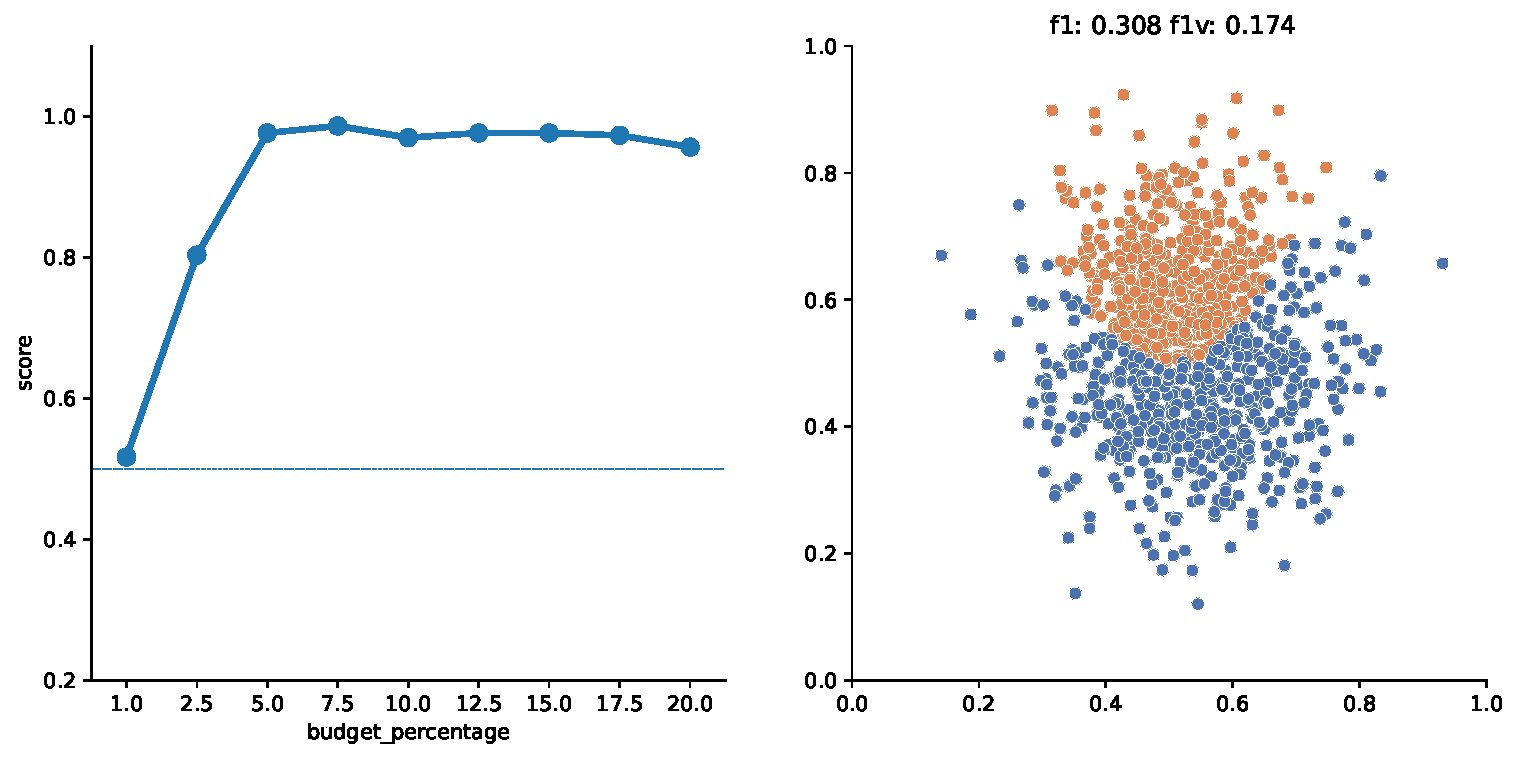
\includegraphics[width=\textwidth]{img/2d_v2/3.pdf}
    \end{subfigure}
    \begin{subfigure}{.5\textwidth}
        \centering
        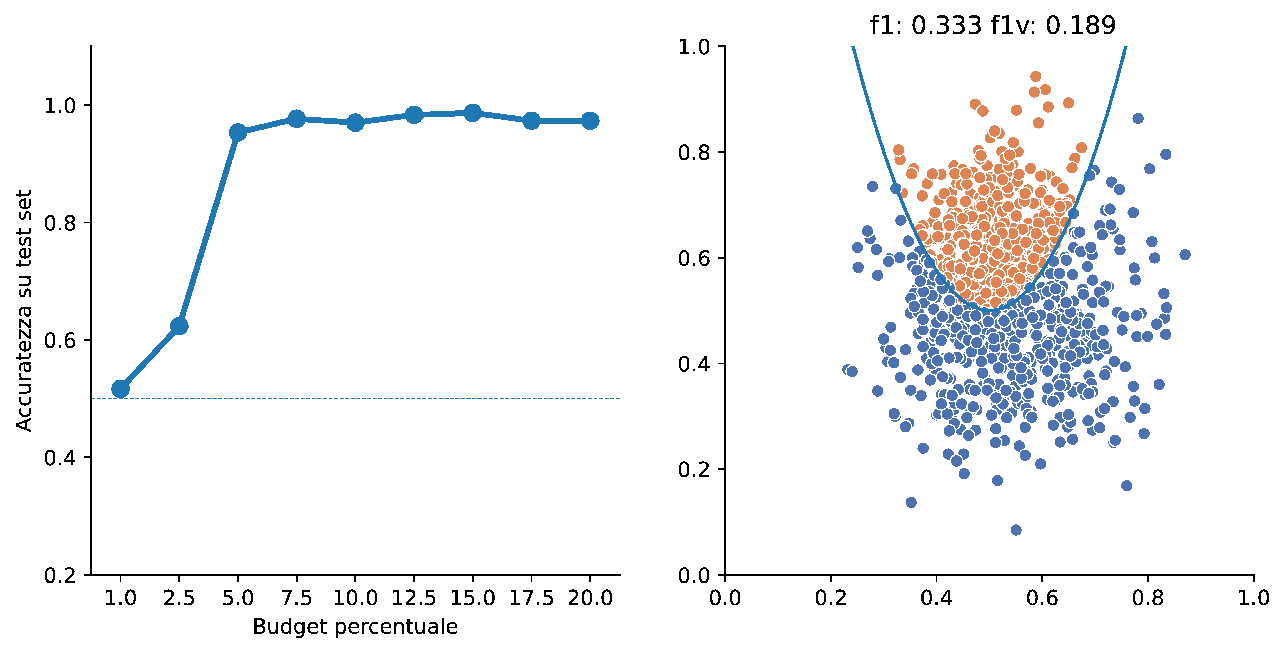
\includegraphics[width=\textwidth]{img/2d_v2/4.pdf}
    \end{subfigure}%
    %
    \hfill
    %
    \begin{subfigure}{.5\textwidth}
        \centering
        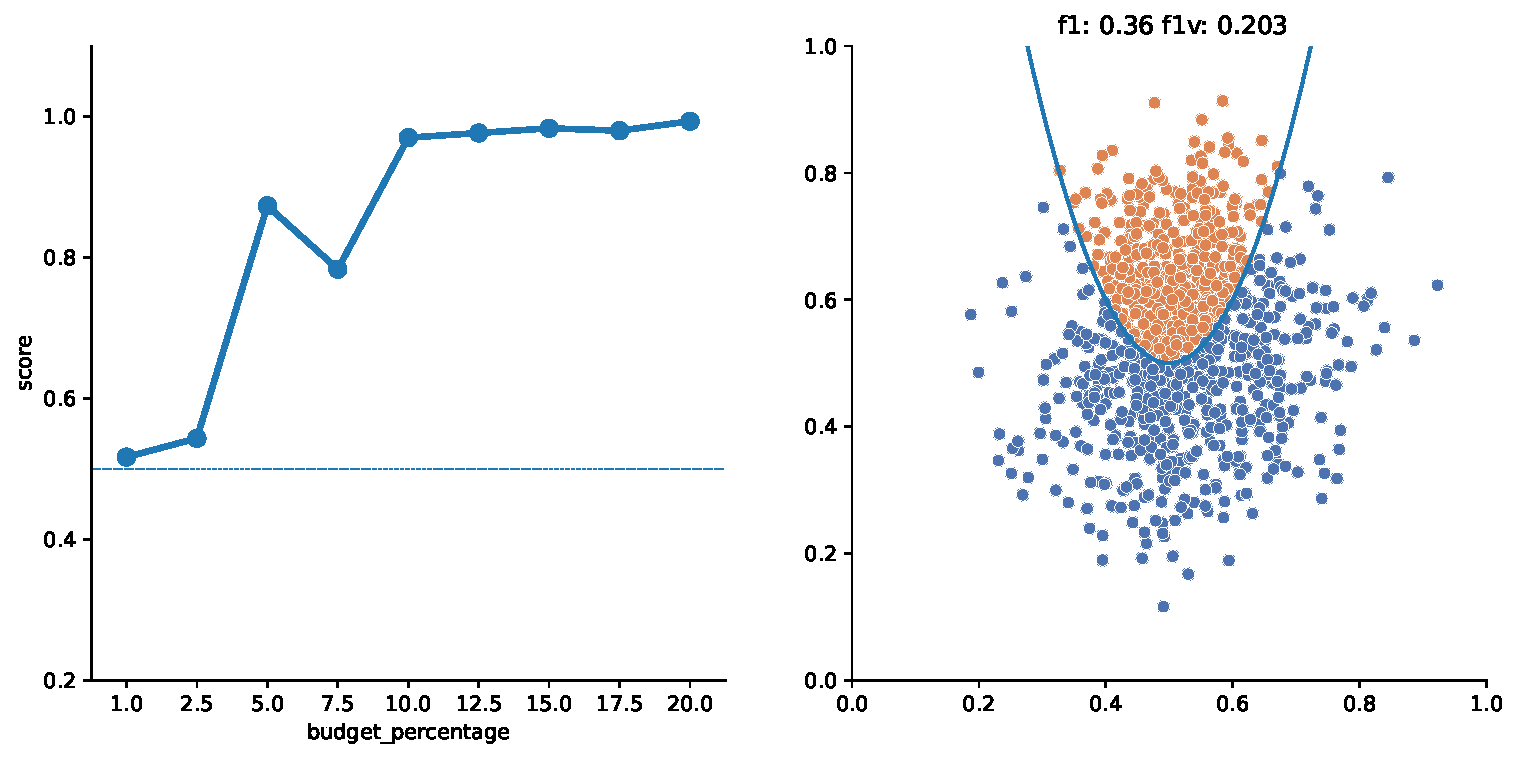
\includegraphics[width=\textwidth]{img/2d_v2/5.pdf}
    \end{subfigure}
    \begin{subfigure}{.5\textwidth}
        \centering
        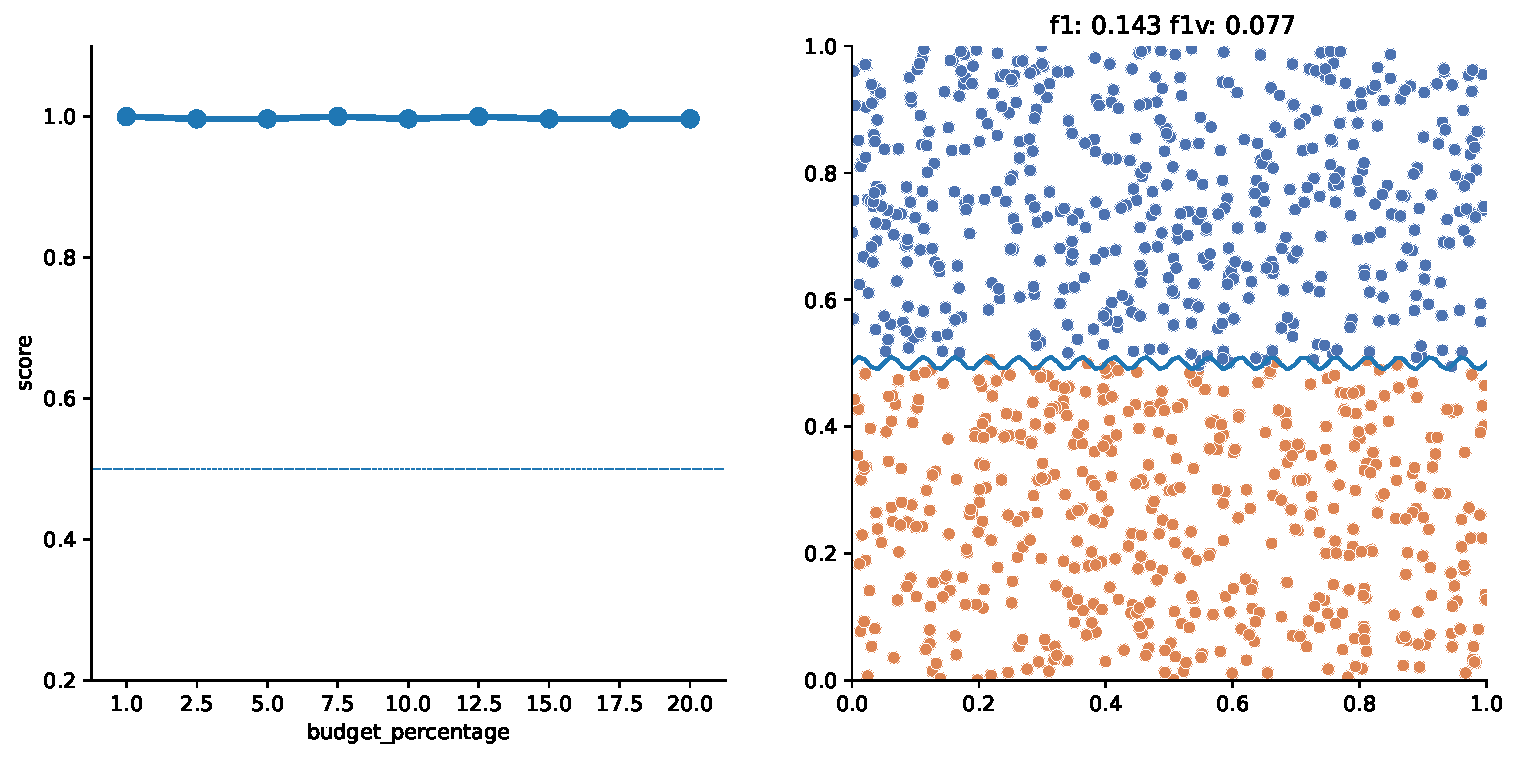
\includegraphics[width=\textwidth]{img/2d_v2/6.pdf}
    \end{subfigure}%
    %
    \hfill
    %
    \begin{subfigure}{.5\textwidth}
        \centering
        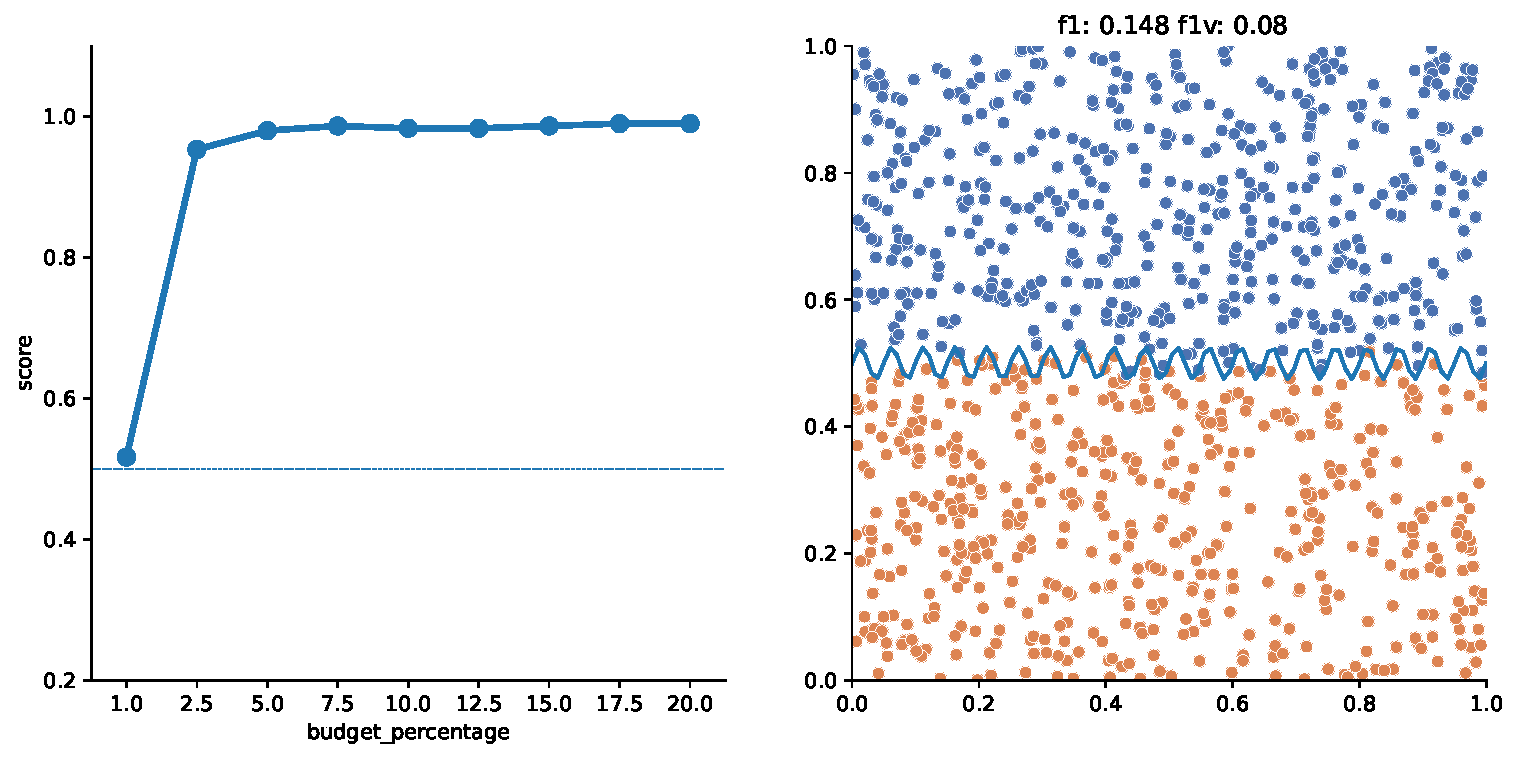
\includegraphics[width=\textwidth]{img/2d_v2/7.pdf}
    \end{subfigure}
    \begin{subfigure}{.5\textwidth}
        \centering
        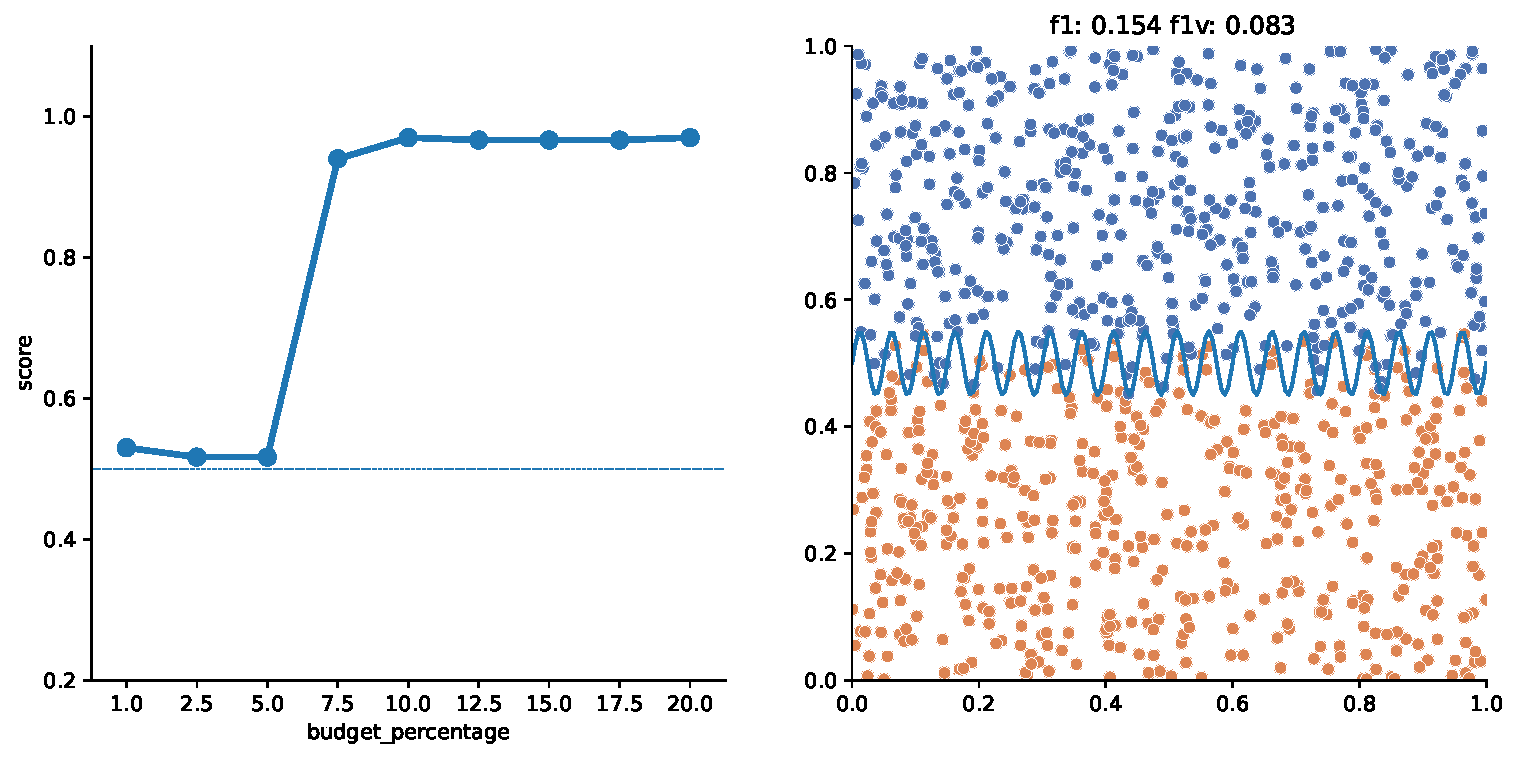
\includegraphics[width=\textwidth]{img/2d_v2/8.pdf}
    \end{subfigure}%
\caption{Esperimenti su dataset sintetici 2D con variazione del budget in funzione della dimensione del dataset. Ognuno dei grafici a sinistra indica l'andamento dell'accuratezza sui dati di \emph{test} al variare del \emph{budget}; ognuno dei grafici a destra rappresenta il dataset utilizzato con le rispettive misure di ``difficoltà''.}
\label{fig:2d_v2_1}
\end{figure}
\begin{figure}
    \begin{subfigure}{.5\textwidth}
        \centering
        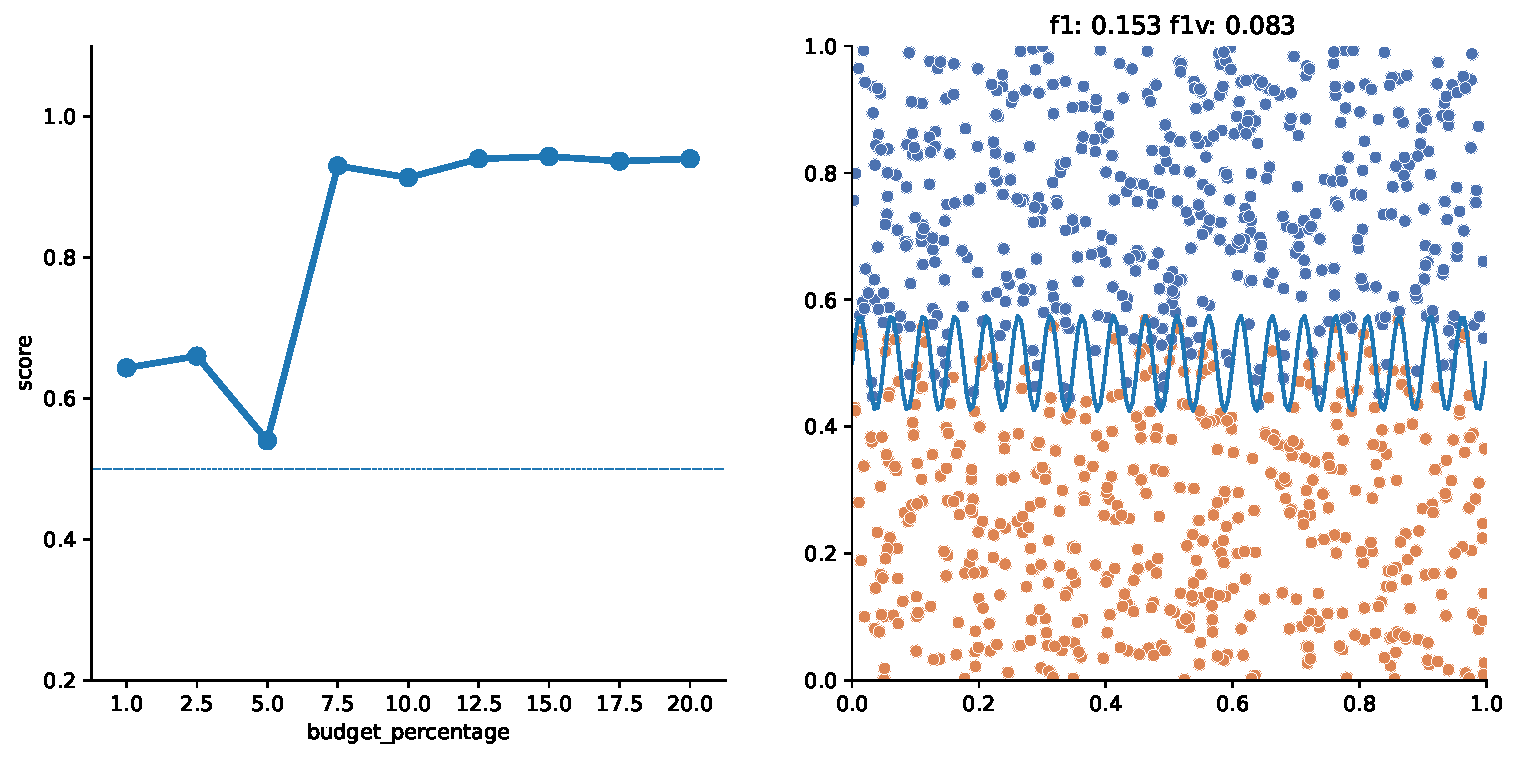
\includegraphics[width=\textwidth]{img/2d_v2/9.pdf}
    \end{subfigure}%
    \begin{subfigure}{.5\textwidth}
        \centering
        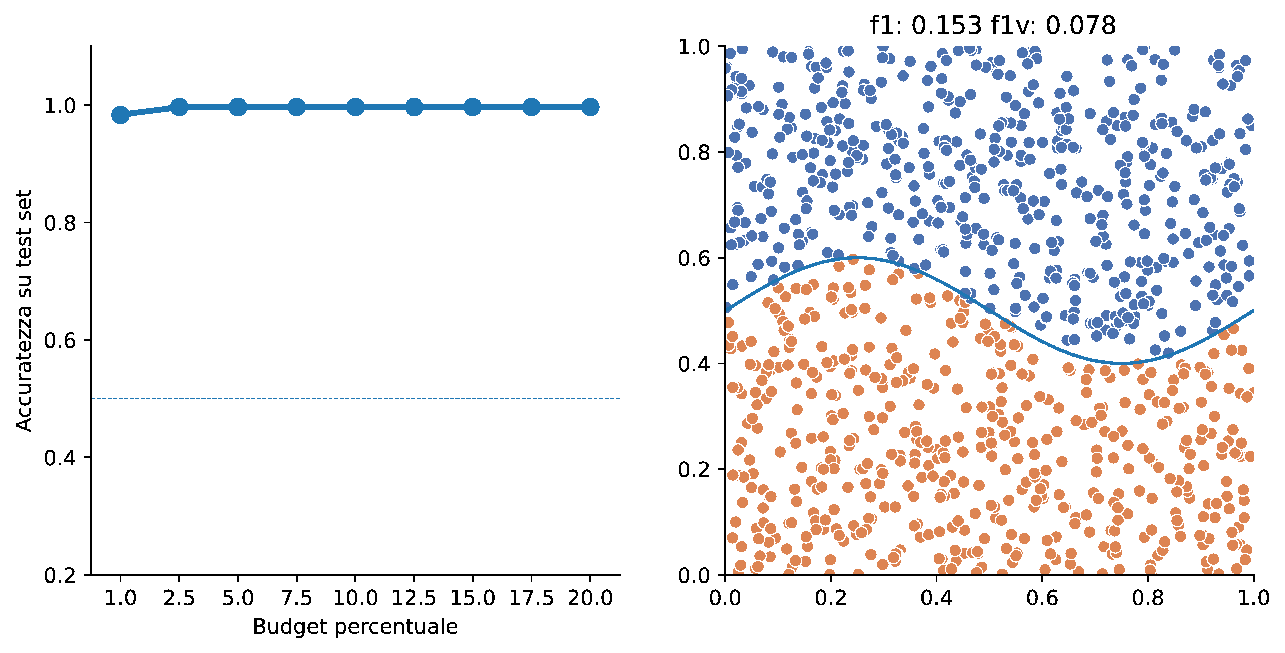
\includegraphics[width=\textwidth]{img/2d_v2/10.pdf}
    \end{subfigure}
    %
    \hfill
    %
    \begin{subfigure}{.5\textwidth}
        \centering
        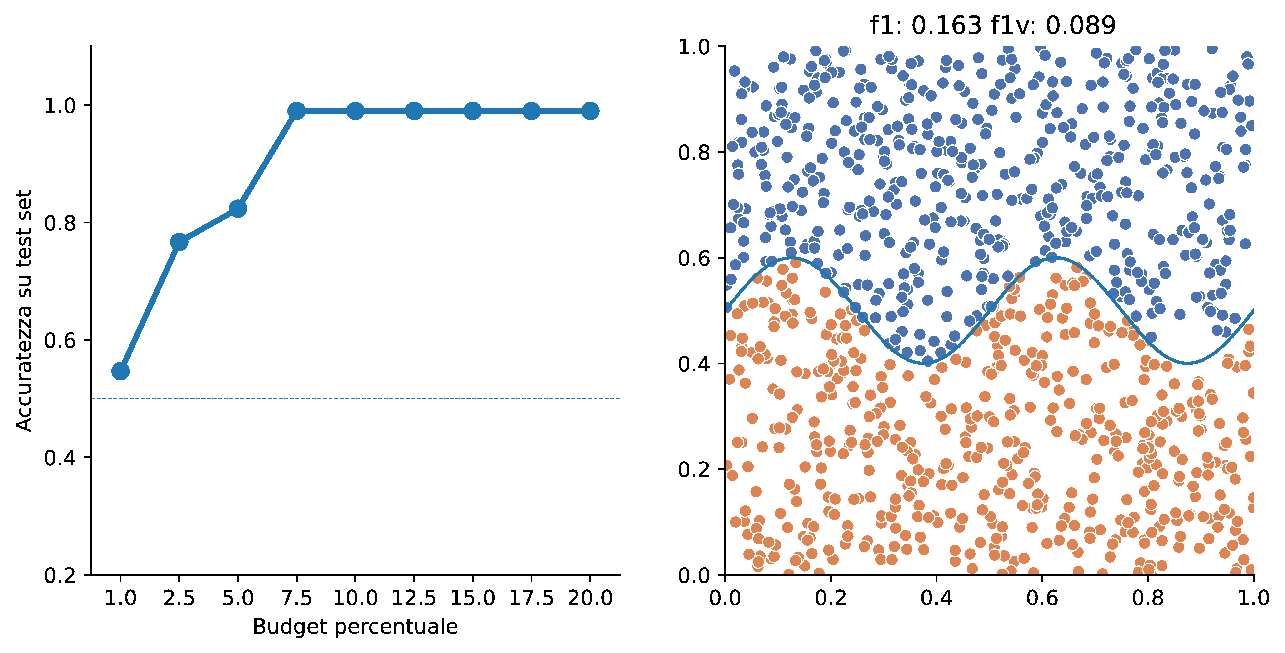
\includegraphics[width=\textwidth]{img/2d_v2/11.pdf}
    \end{subfigure}
    \begin{subfigure}{.5\textwidth}
        \centering
        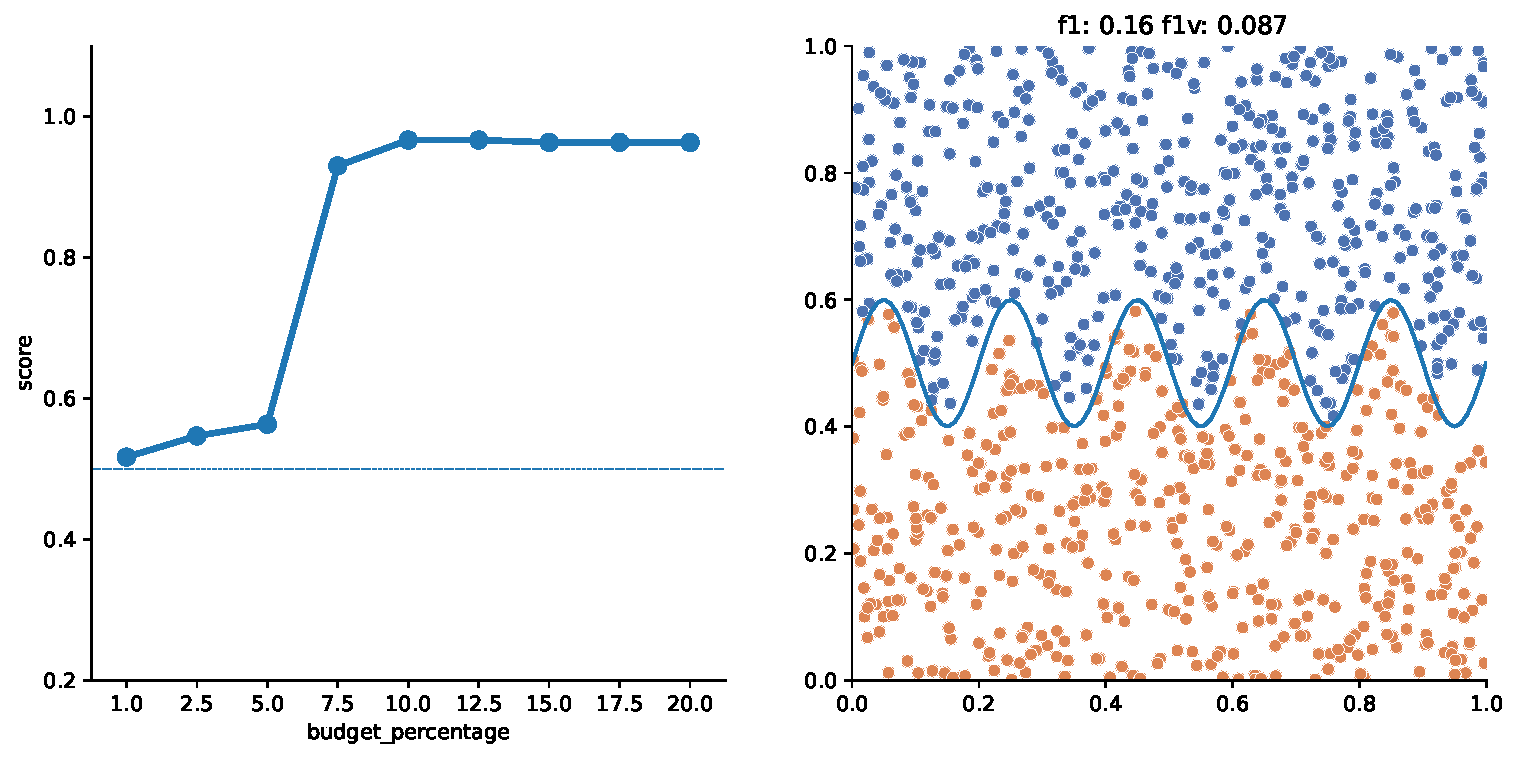
\includegraphics[width=\textwidth]{img/2d_v2/12.pdf}
    \end{subfigure}%
    %
    \hfill
    %
    \begin{subfigure}{.5\textwidth}
        \centering
        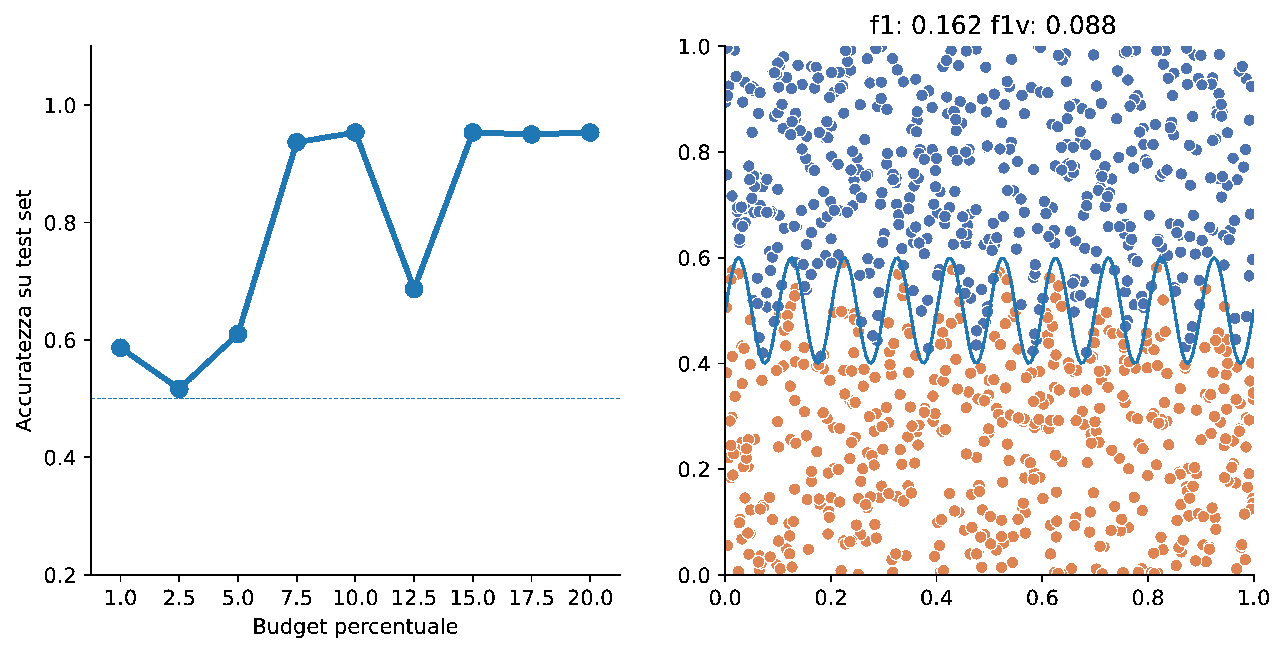
\includegraphics[width=\textwidth]{img/2d_v2/13.pdf}
    \end{subfigure}
    \begin{subfigure}{.5\textwidth}
        \centering
        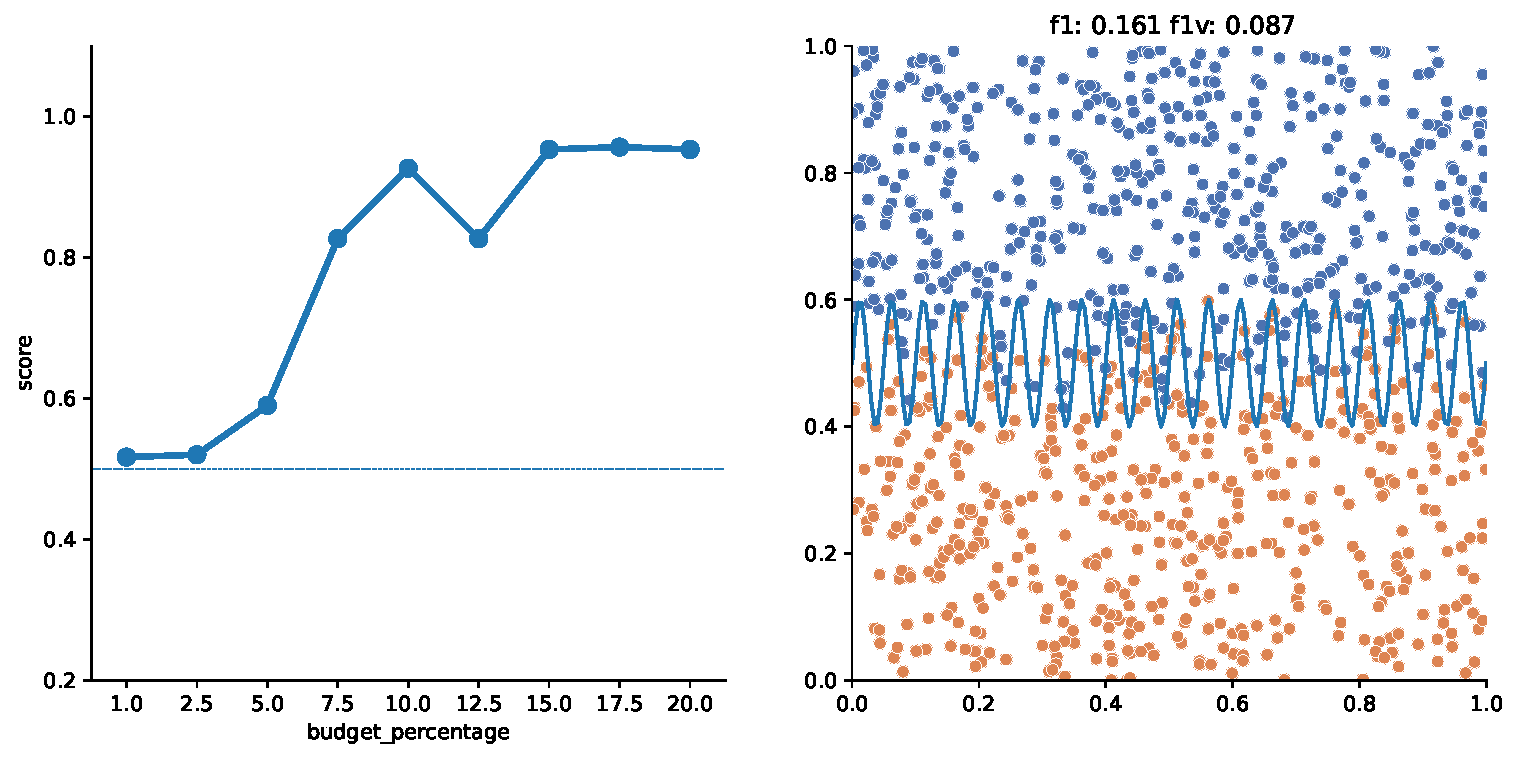
\includegraphics[width=\textwidth]{img/2d_v2/14.pdf}
    \end{subfigure}%
    %
    \hfill
    %
    \begin{subfigure}{.5\textwidth}
        \centering
        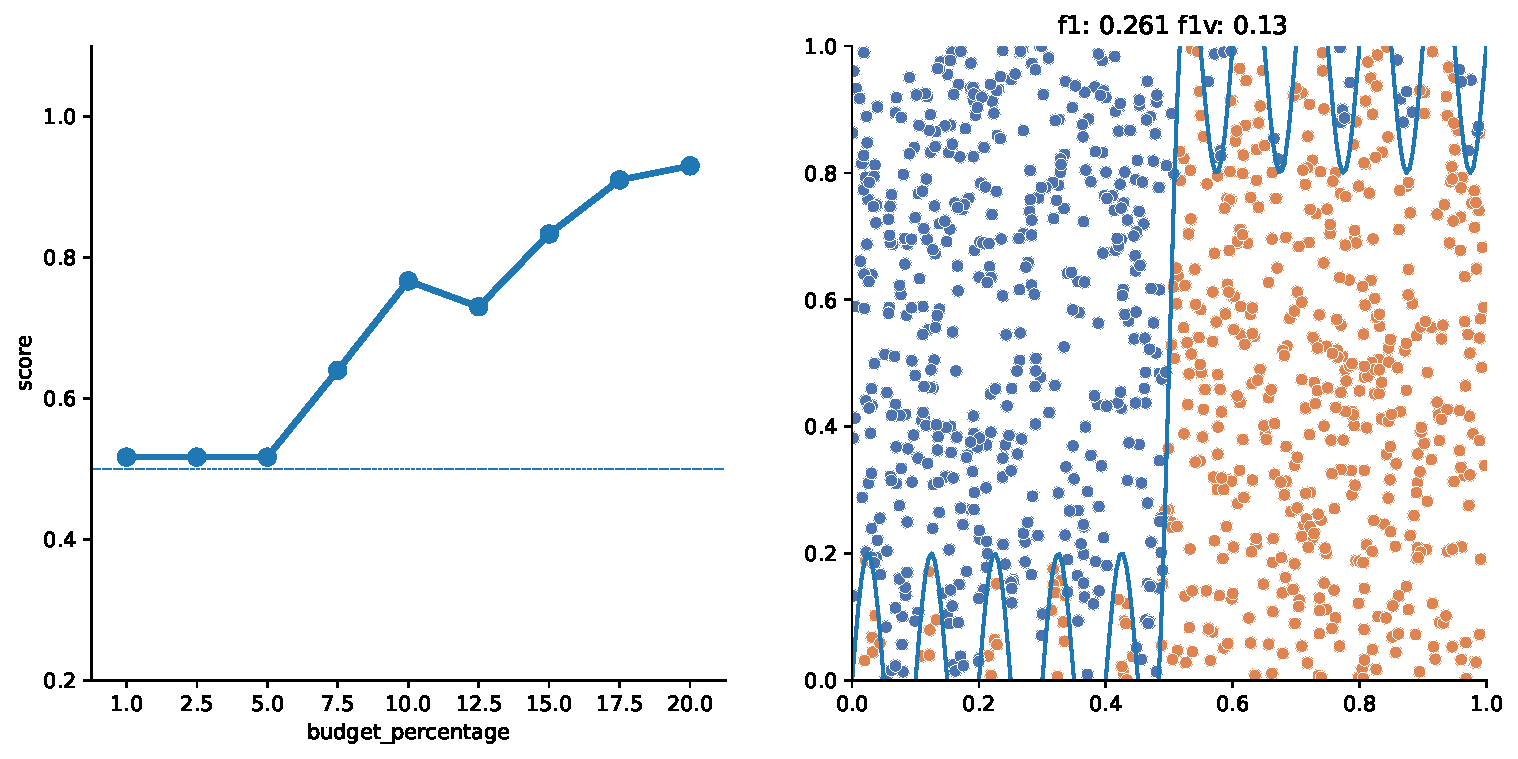
\includegraphics[width=\textwidth]{img/2d_v2/15.pdf}
    \end{subfigure}
\caption{Esperimenti su dataset sintetici 2D con variazione del budget in funzione della dimensione del dataset. Ognuno dei grafici a sinistra indica l'andamento dell'accuratezza sui dati di \emph{test} al variare del \emph{budget}; ognuno dei grafici a destra rappresenta il dataset utilizzato con le rispettive misure di ``difficoltà''.}
\label{fig:2d_v2_2}
\end{figure}   

Dai risultati ottenuti possiamo vedere come anche per la maggior parte dei dataset ``difficili'' si possa utilizzare un \emph{budget} stringente, tra il $7\%$ ed il $10\%$, con perdite accettabili di accuratezza.
Per dataset di fatto linearmente separabili la riduzione di budget può essere molto importante, anche con solo l'$1\%$ del dataset si ottiene accuratezza pari a quella ottenuta con \emph{budget} molto più alti.

%\subsection{Esperimenti su dataset con rumore}

\section{Esperimenti su dataset sintetici 3D}\label{sec:exp:synth_3d}
Una piccola parte degli esperimenti è stata effettuata su dataset in 3 dimensioni con 5600 dati di addestramento e 2400 di test.
La strategia utilizzata è quella di impostare il \emph{budegt} in funzione del numero di vettori di supporto di un modello classico. 
In~\Cref{fig:3d_exp} si possono vedere i risultati ottenuti e i dataset utilizzati.
\begin{figure}
    \begin{subfigure}{\textwidth}
        \centering
        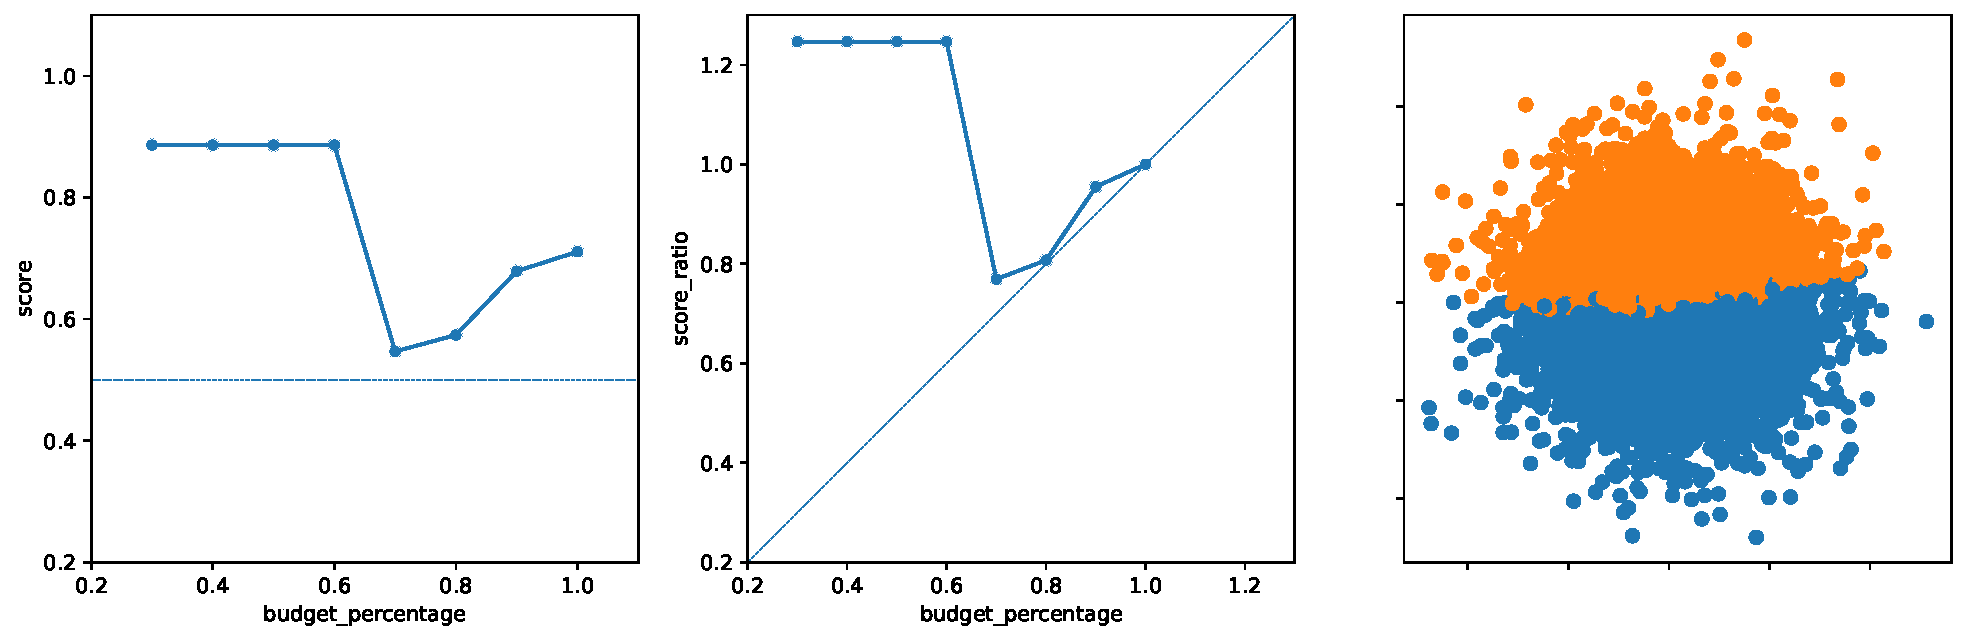
\includegraphics[width=\textwidth]{img/3d/1.pdf}
    \end{subfigure}%
    \hfill
    \begin{subfigure}{\textwidth}
        \centering
        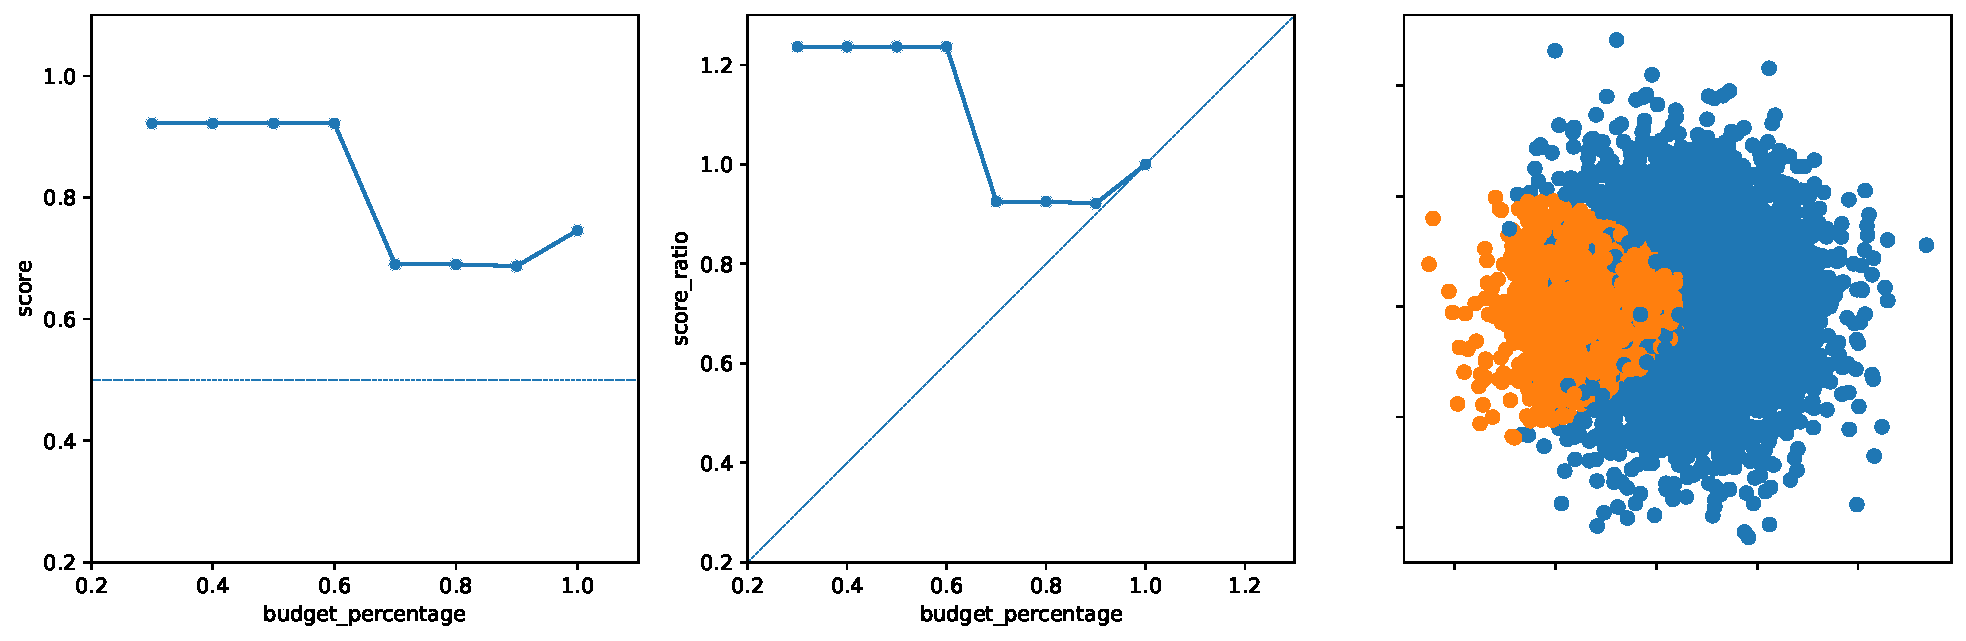
\includegraphics[width=\textwidth]{img/3d/2.pdf}
    \end{subfigure}%
    \hfill
    \begin{subfigure}{\textwidth}
        \centering
        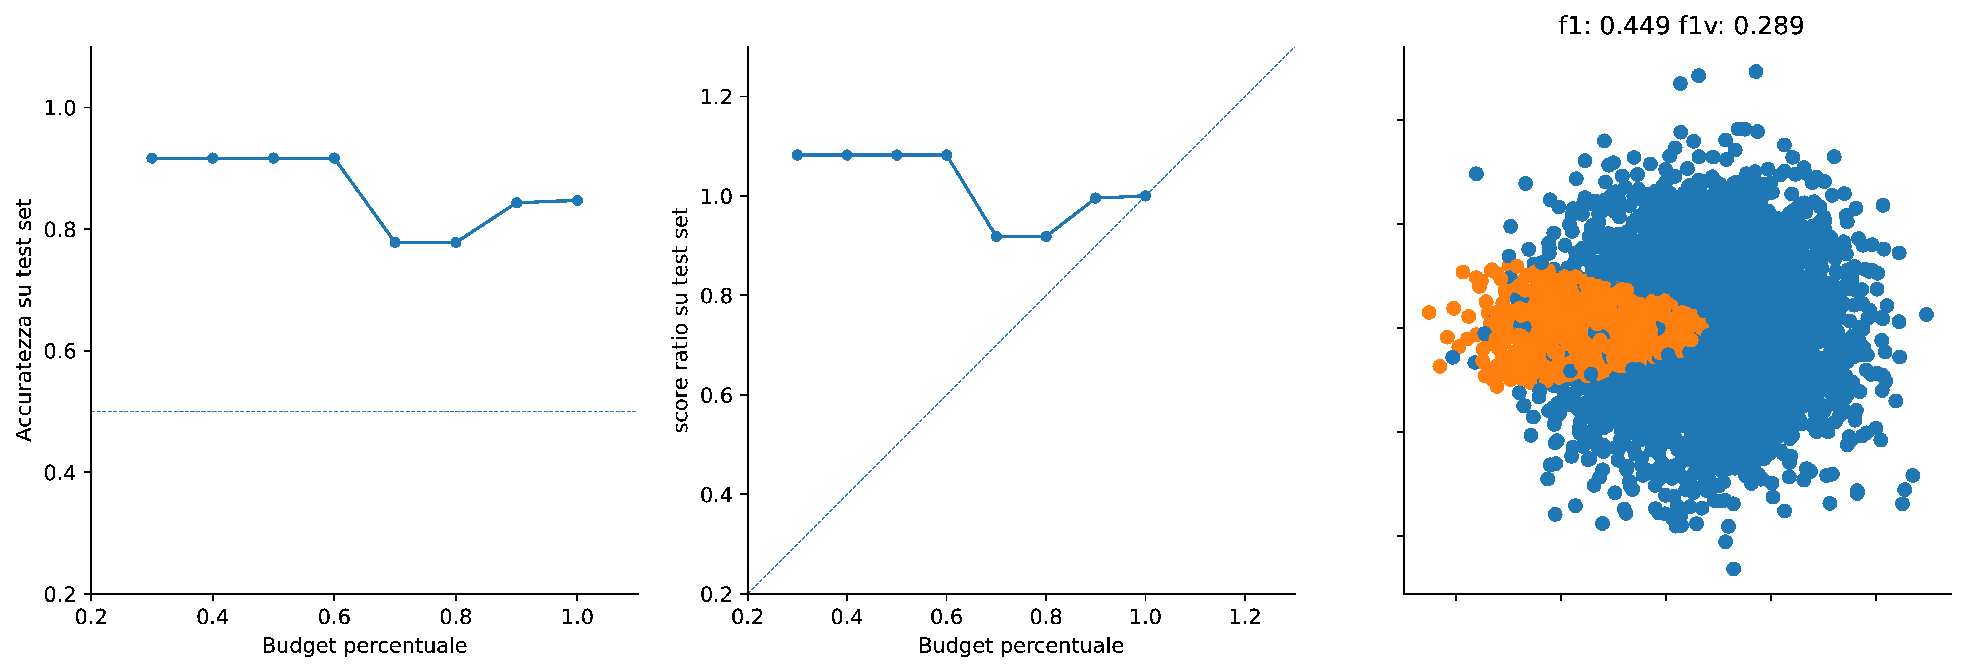
\includegraphics[width=\textwidth]{img/3d/3.pdf}
    \end{subfigure}%
\caption{Esperimenti su dataset sintetici 3D con variazione del budget rispetto ad un modello classico. A sinistra l'accuratezza sui dati di test al variare del budget; al centro lo ``score ratio'' al variare del budget; a destra il dataset ridotto a due dimensioni utilizzando \emph{principal component analysis}.}
\label{fig:3d_exp}
\end{figure}
Per limitare la quantità di tempo e risorse richiesti per eseguire questo tipo di esperimenti sono stati utilizzati solamente 3 dataset.

Dai risultati ottenuti possiamo comunque notare come restrizioni di budget significative risultino addirittura in migliori performance rispetto al modello nella formulazione classica. 
Analizzando i modelli ottenuti però si nota come il numero di vettori di supporto nella formulazione classica sia molto elevato (5550, 5592, 5600), praticamente l'intero insieme di dati di addestramento.


\section{Esperimenti su dataset di terze parti}\label{sec:exp:real_ds}
Utilizzando i dataset descritti nella~\Cref{tab:uci_datasets} sono stati ripetuti gli stessi esperimenti effettuati sui dataset sintetici, esprimendo il budget sia in funzione di un modello classico senza vincolo e sia come frazione dei punti del dataset.

I risultati ottenuti esprimendo le variazioni di budget in funzione del modello classico sono visualizzabili in~\Cref{fig:TP_old_strategy}.
\begin{figure}
    \centering
    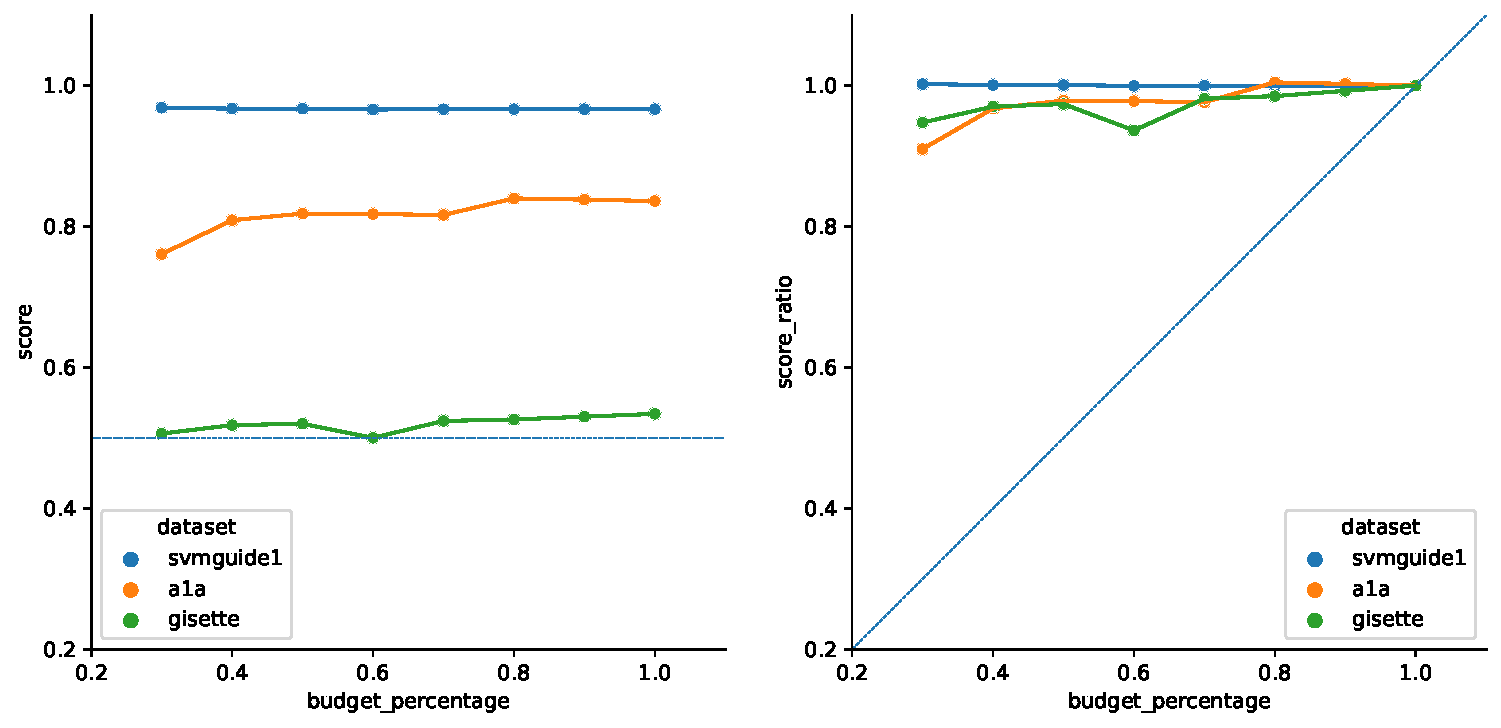
\includegraphics[width=1\linewidth]{img//TP/tp_old_strategy.pdf}
    \caption{Risultati esperimenti su dataset di terze parti con variazione del budget rispetto ad un modello classico. A sinistra l'accuratezza sui dati di test al variare del budget; a destra lo ``score ratio'' al variare del budget.}
    \label{fig:TP_old_strategy}
\end{figure}
Possiamo notare come su questi dataset tutte le riduzioni di budget testate siano efficaci e non risultino in nessuna perdita di accuratezza.

I risultati ottenuti esprimendo le variazioni di budget in funzione della dimensione del dataset sono visualizzabili in~\Cref{fig:TP_new_strategy}.
\begin{figure}
    \centering
    %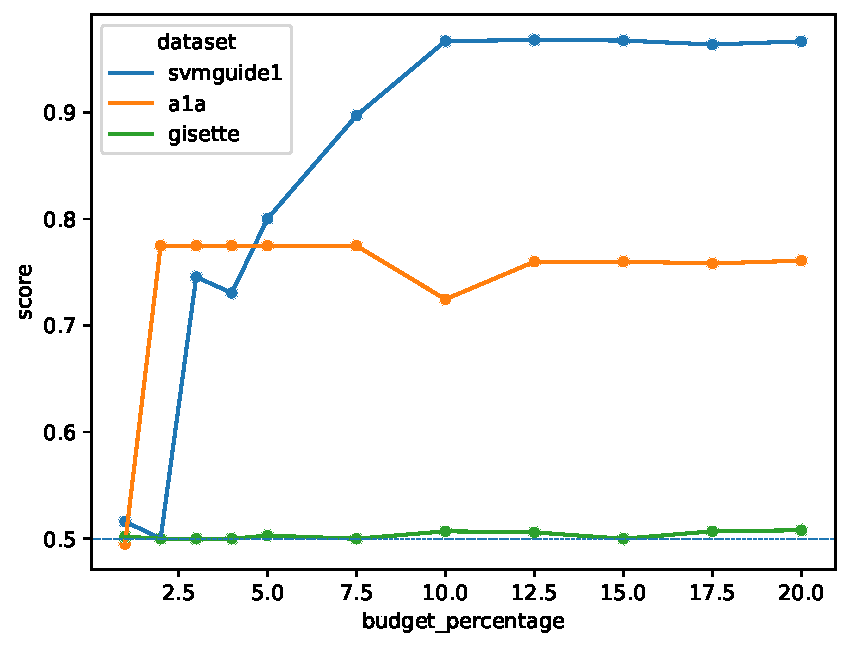
\includegraphics[width=1\linewidth]{img//TP/tp_new_strategy.pdf}
    \caption{Risultati esperimenti su dataset di terze parti con variazione del budget rispetto alla dimensione del dataset. Accuratezza su dati di test al variare del budget}
    \label{fig:TP_new_strategy}
\end{figure}
Possiamo notare come ::::::::::::::************************

\section{Comparazione con altri metodi}\label{sec:comparazione_metodi}
Per meglio inquadrare i risultati ottenuti dal metodo proposto in questa tesi, son stati ripetuti gli esperimenti effettuati utilizzando delle implementazioni di metodi proposti in letteratura e visti nel~\Cref{chap:sparse_svc}, in particolare:
\begin{itemize}
    \item \emph{BSGD SVM} esposto in~\cite{2012_bsgd}. Risolutore basato su discesa del gradiente che mantiene una dimensione massima dell'insieme dei vettori di supporto utilizzando la strategia di unione o rimozione.
    \item \emph{NSSVM} esposto in~\cite{2020_sparse_svm}. Risolutore basato su \emph{Newton method} che minimizza il numero di vettori di supporto tramite una funzione di costo adatta.
    % \item \emph{LIB IRWLS} esposto in~\cite{LIBIRWLS}. Risolutore parallelo basato su un approssimazione \emph{greedy} della matrice \emph{kernel} e utilizzo dell'algoritmo IRWLS~\cite{IRWLS}
\end{itemize}
Utilizzando gli stessi dataset sintetici generati con i parametri nelle~\Cref{tab:parametri_ds_sin,tab:parametri_ds_pacman} e utilizzando \emph{5-fold cross-validation grid search} con una griglia di parametri adatti (\Cref{tab:gridsearch_comparazioni}), viene misurata l'accuratezza sui dati di \emph{test} per gli stessi valori di \emph{budget} utilizzati in precedenza.
\begin{table}
    \centering
    \begin{tabular}{ccccc}
        \toprule
        Algoritmo & $C$ & \emph{Kernel} & $\gamma$ & d \\
        \midrule
        \multirow{2}{*}{BSGD}   & \multirow{2}{*}{/}  & Gaussiano   & [0.001, 0.01, 0.1, 1, 10]   & /\\
                                      \cline{3-5}
                                &   & Polinomiale & / & [2, 5, 10] \\
        \hline
        NSSVM   & / & / & / & / \\
        % \hline
        % IRWLS   & [0.01, 0.1, 1, 10]  & Gaussiano & [0.001, 0.01, 0.1, 1, 10] & / \\
        \bottomrule
    \end{tabular}
    \caption{Parametri \emph{grid search} per gli algoritmi presenti in letteratura.}
    \label{tab:gridsearch_comparazioni}
\end{table}
Nelle~\Cref{fig:comp_old_1,fig:comp_old_2} si possono vedere i valori di accuratezza ottenuti da questi metodi definendo il budget in funzione di un modello classico e confrontati con i risultati ottenuti con \emph{budgeted SVC} e i dataset utilizzati.
\begin{figure}
    \begin{subfigure}{.5\textwidth}
        \centering
        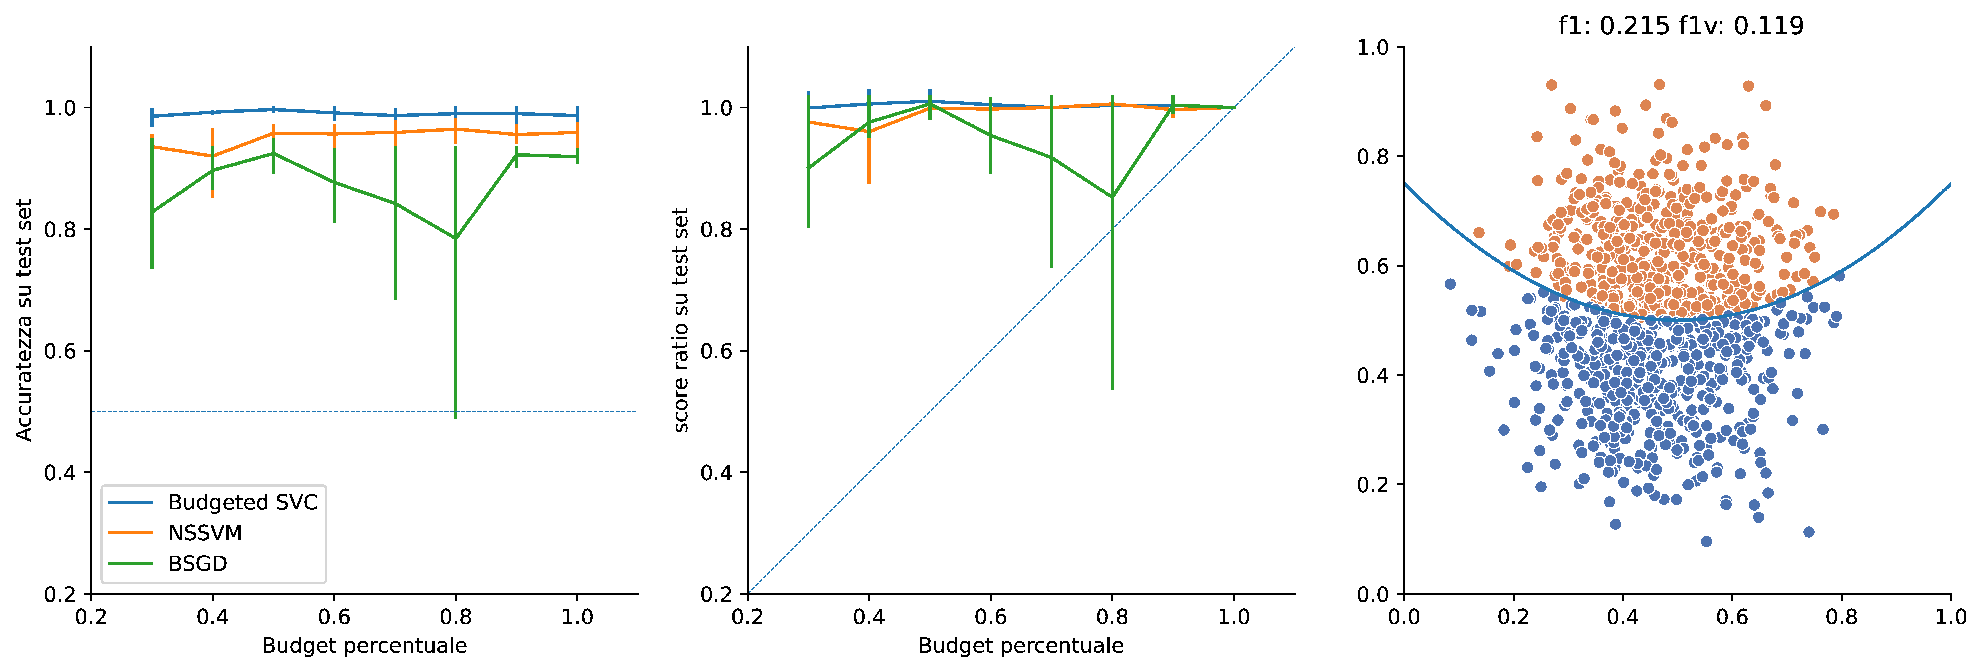
\includegraphics[width=\textwidth]{img/comp_old/1.pdf}
    \end{subfigure}%
    \begin{subfigure}{.5\textwidth}
        \centering
        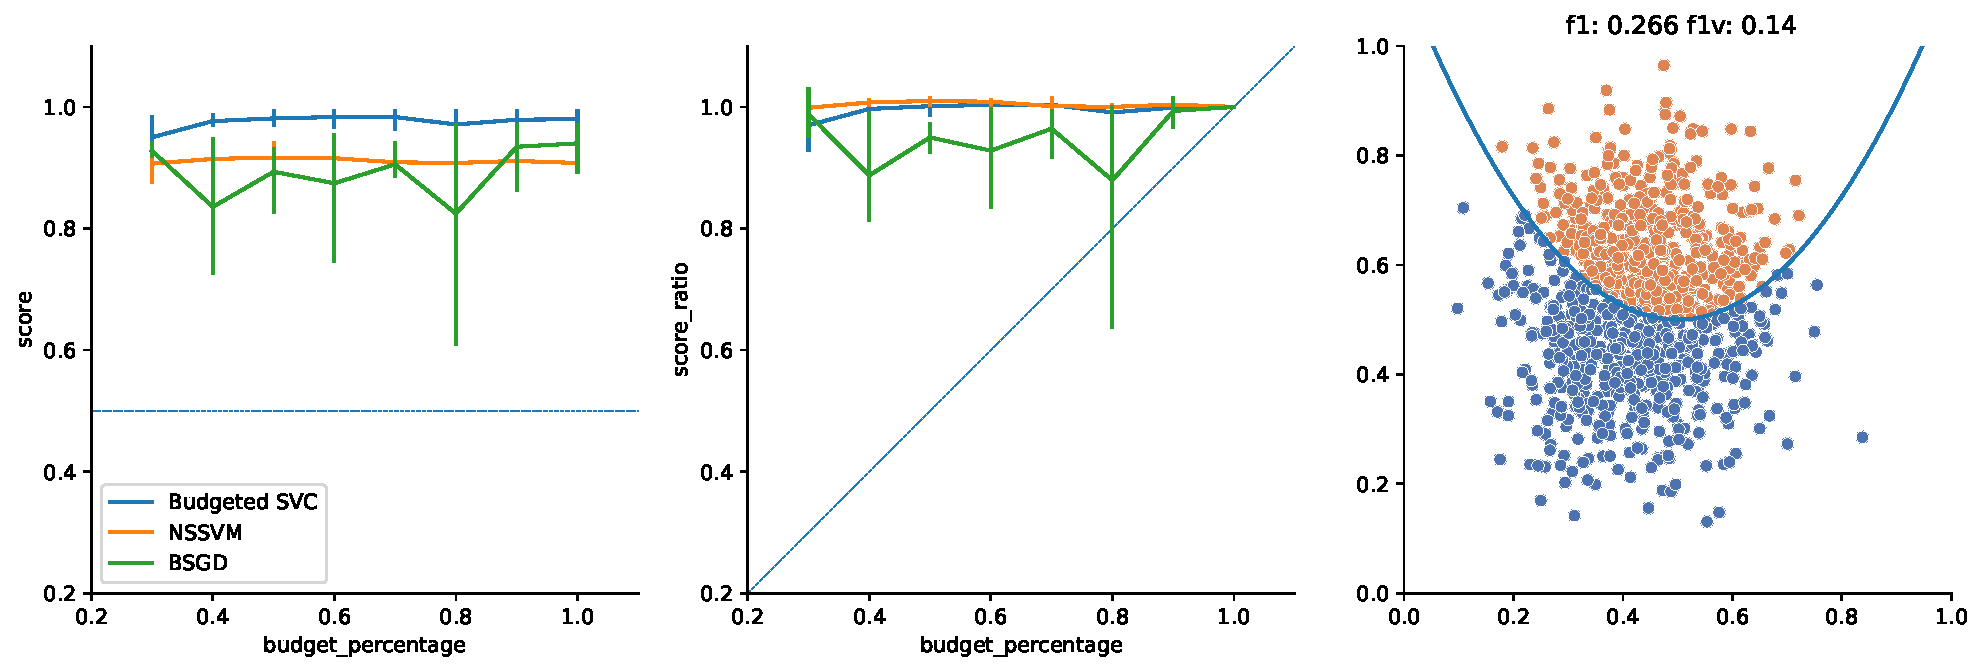
\includegraphics[width=\textwidth]{img/comp_old/2.pdf}
    \end{subfigure}
    %
    \hfill
    %
    \begin{subfigure}{.5\textwidth}
        \centering
        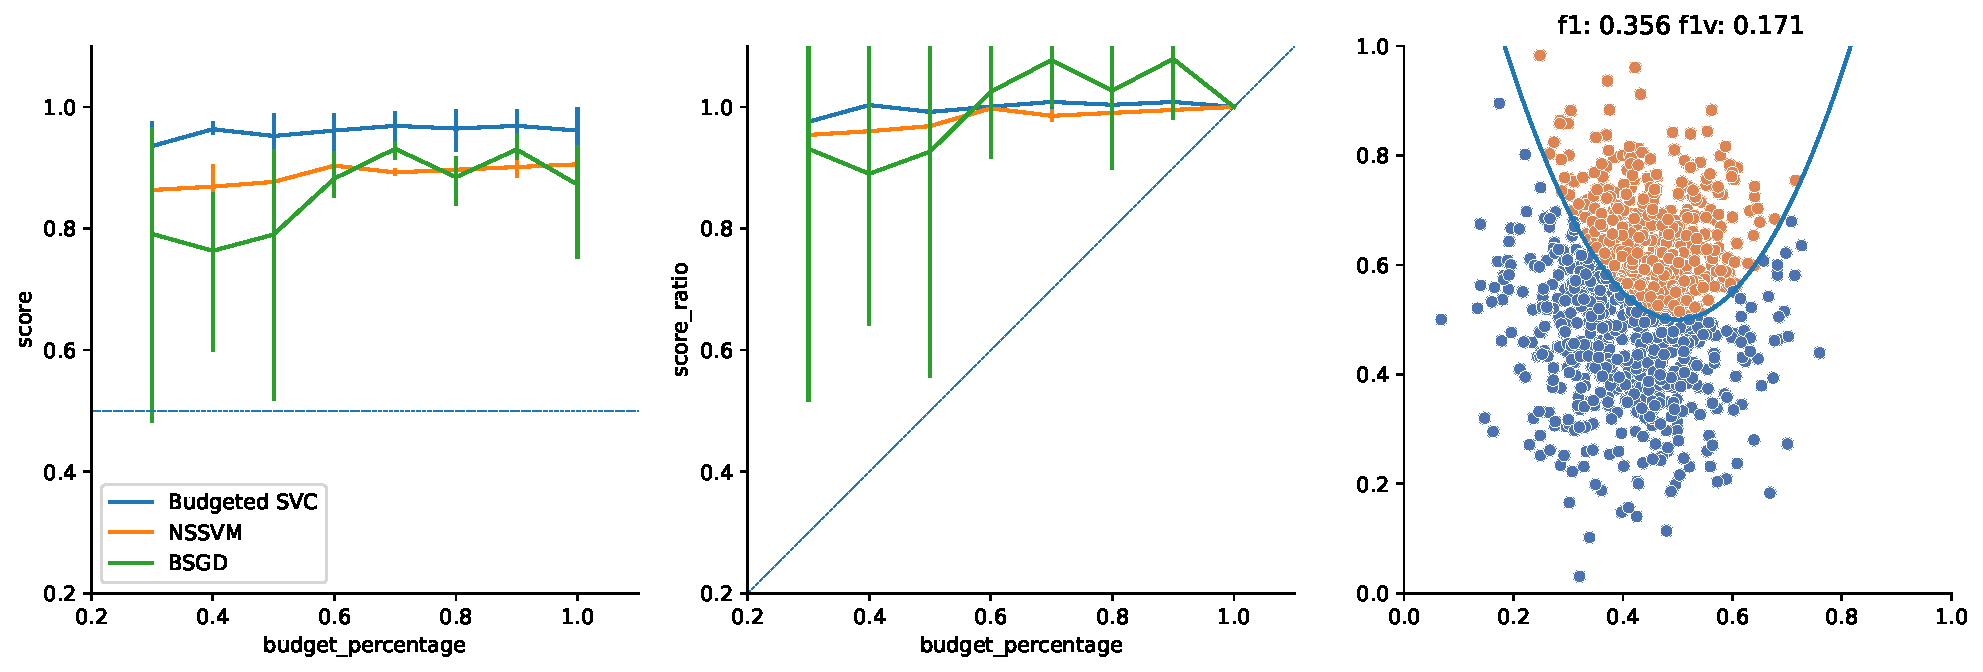
\includegraphics[width=\textwidth]{img/comp_old/3.pdf}
    \end{subfigure}
    \begin{subfigure}{.5\textwidth}
        \centering
        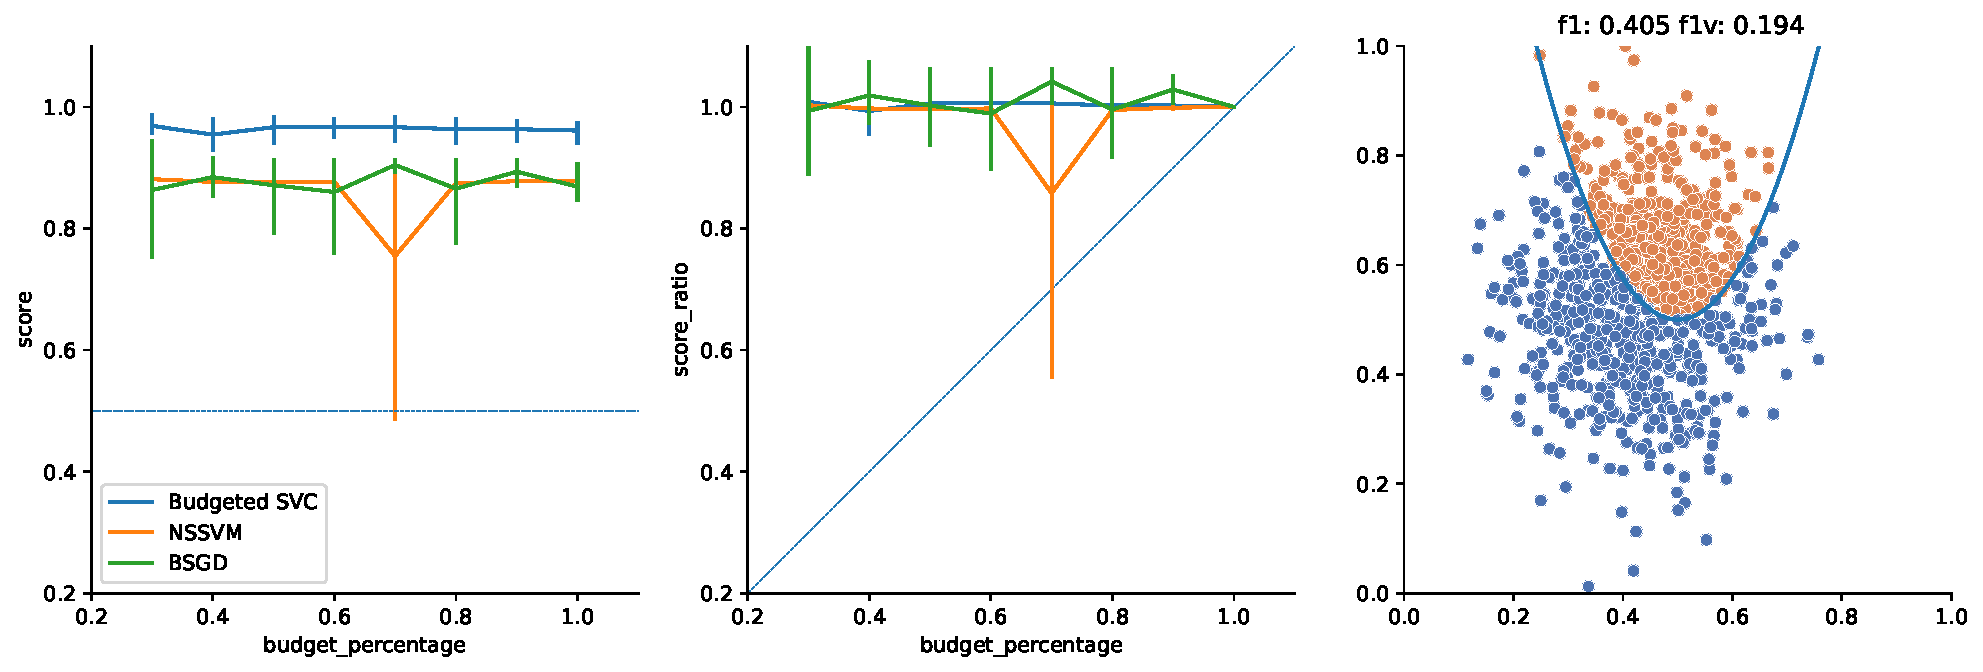
\includegraphics[width=\textwidth]{img/comp_old/4.pdf}
    \end{subfigure}%
    %
    \hfill
    %
    \begin{subfigure}{.5\textwidth}
        \centering
        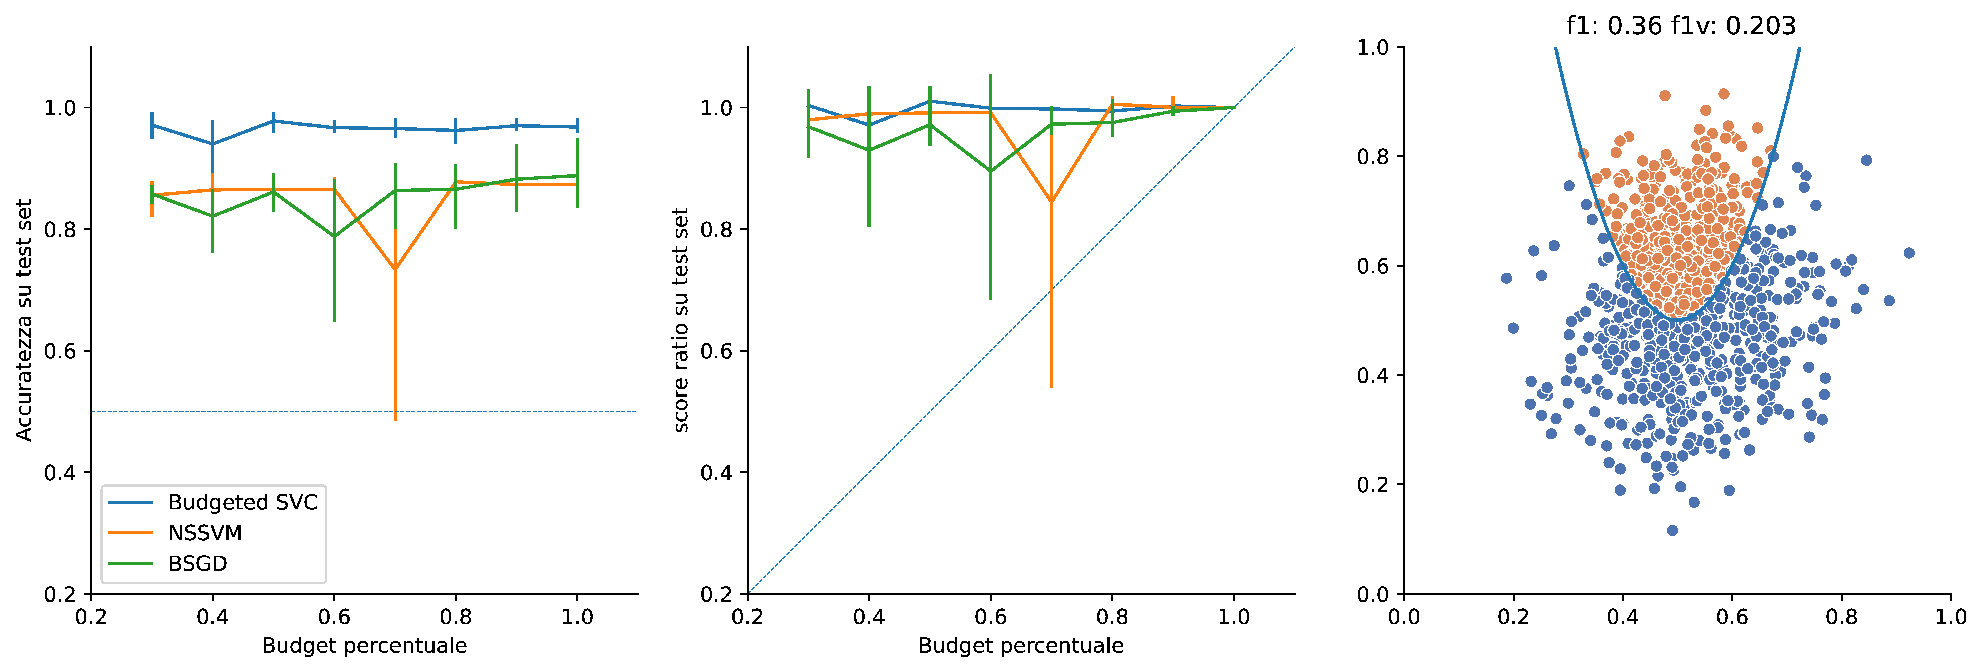
\includegraphics[width=\textwidth]{img/comp_old/5.pdf}
    \end{subfigure}
    \begin{subfigure}{.5\textwidth}
        \centering
        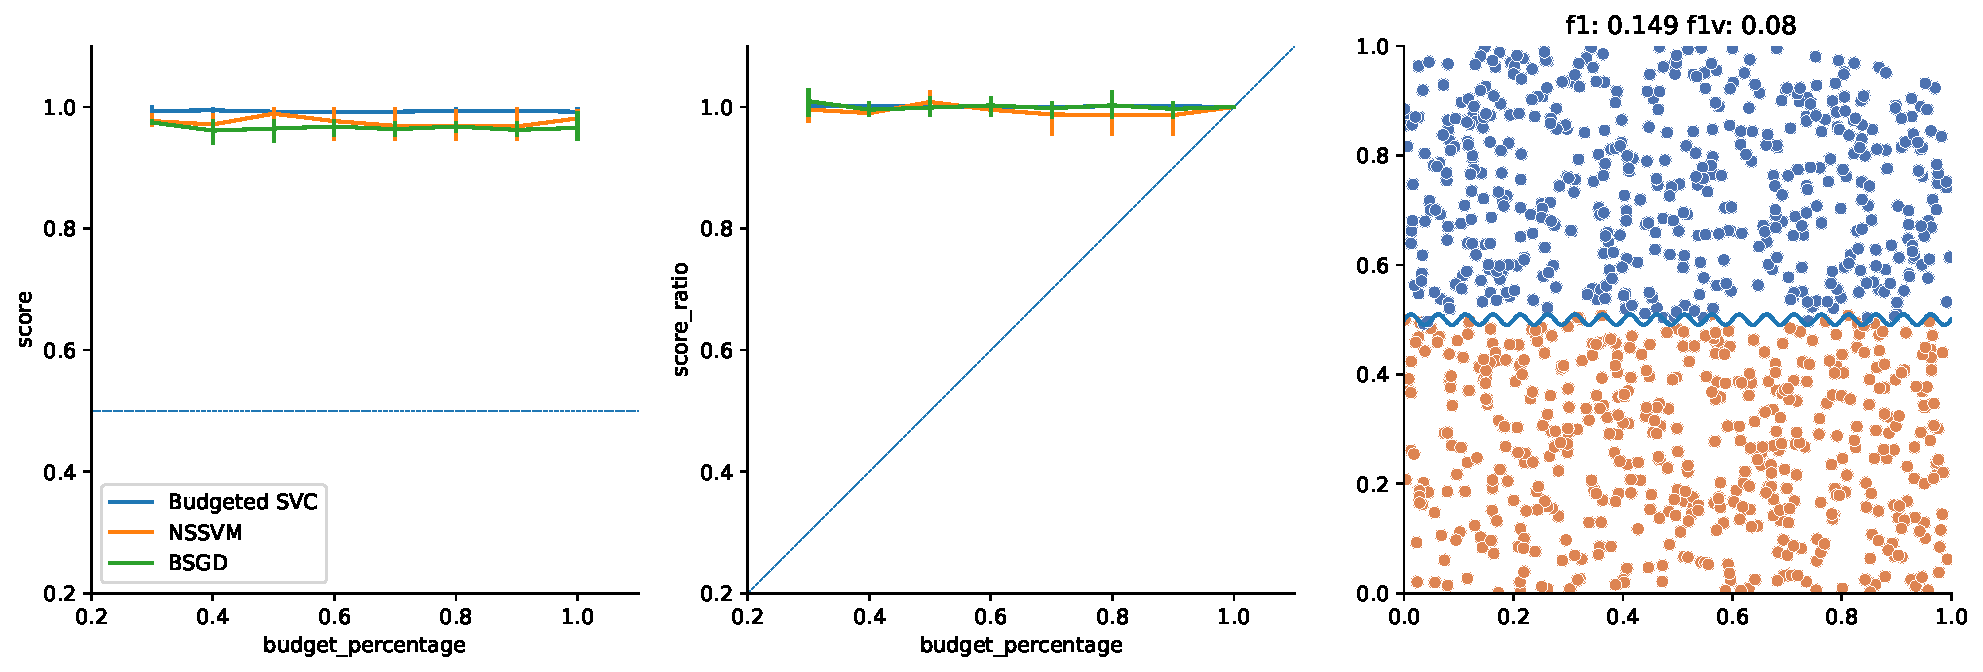
\includegraphics[width=\textwidth]{img/comp_old/6.pdf}
    \end{subfigure}%
    %
    \hfill
    %
    \begin{subfigure}{.5\textwidth}
        \centering
        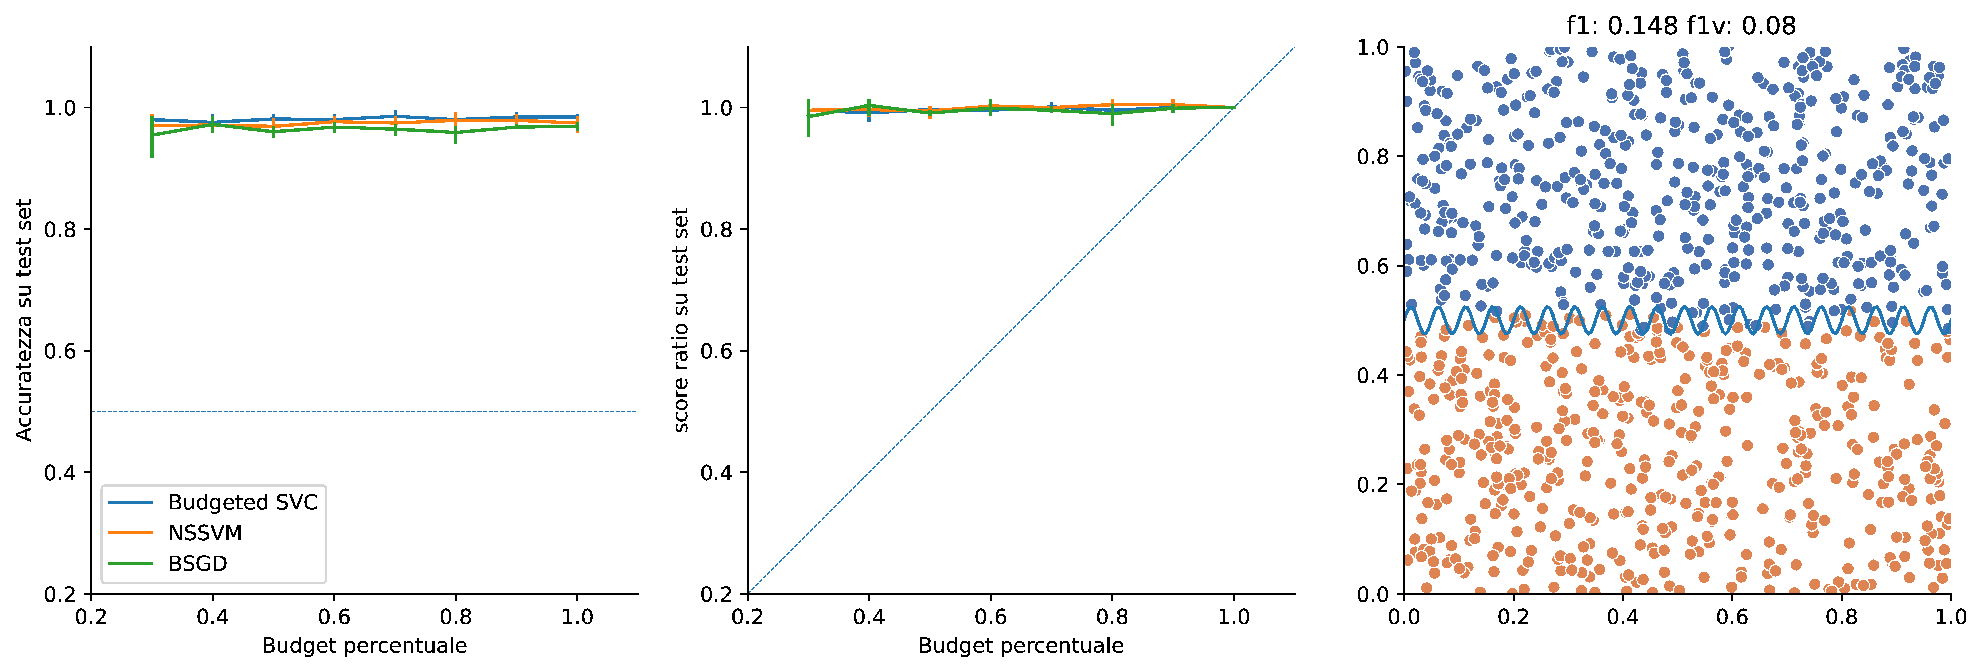
\includegraphics[width=\textwidth]{img/comp_old/7.pdf}
    \end{subfigure}
    \begin{subfigure}{.5\textwidth}
        \centering
        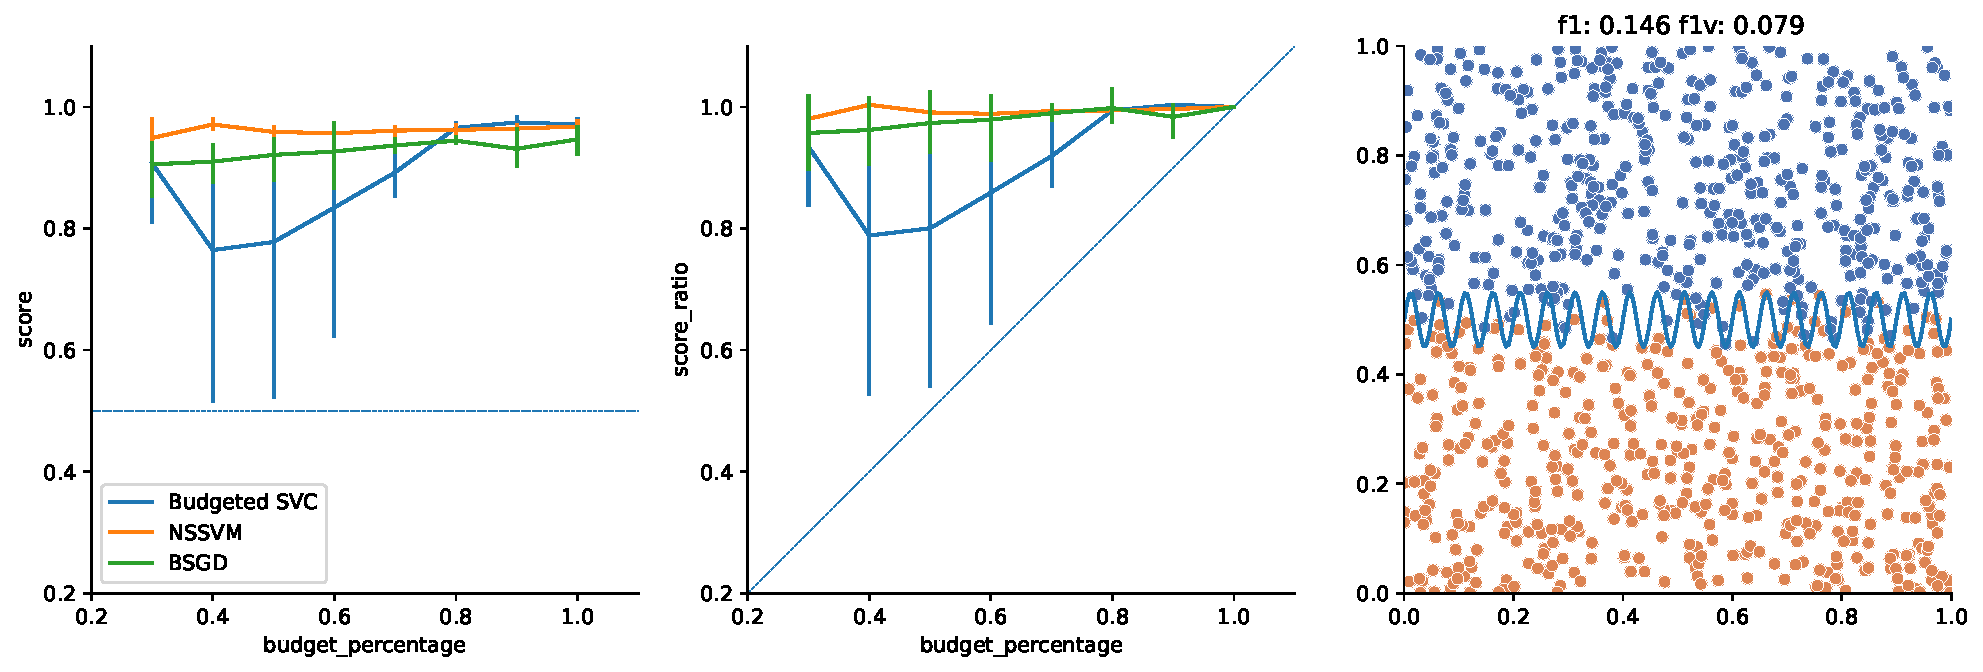
\includegraphics[width=\textwidth]{img/comp_old/8.pdf}
    \end{subfigure}
\caption{Esperimenti su dataset sintetici 2D con variazione del budget in funzione della dimensione del dataset, analogo ai risultati in~\Cref{fig:risultati_2d_1,fig:risultati_2d_2} ma con una curva ogni metodo utilizzato: la proposta \emph{Budgeted SVC}, i metodi \emph{NSSVM} e \emph{BSGD}.}
\label{fig:comp_old_1}
\end{figure}   
\begin{figure}
    \begin{subfigure}{.5\textwidth}
        \centering
        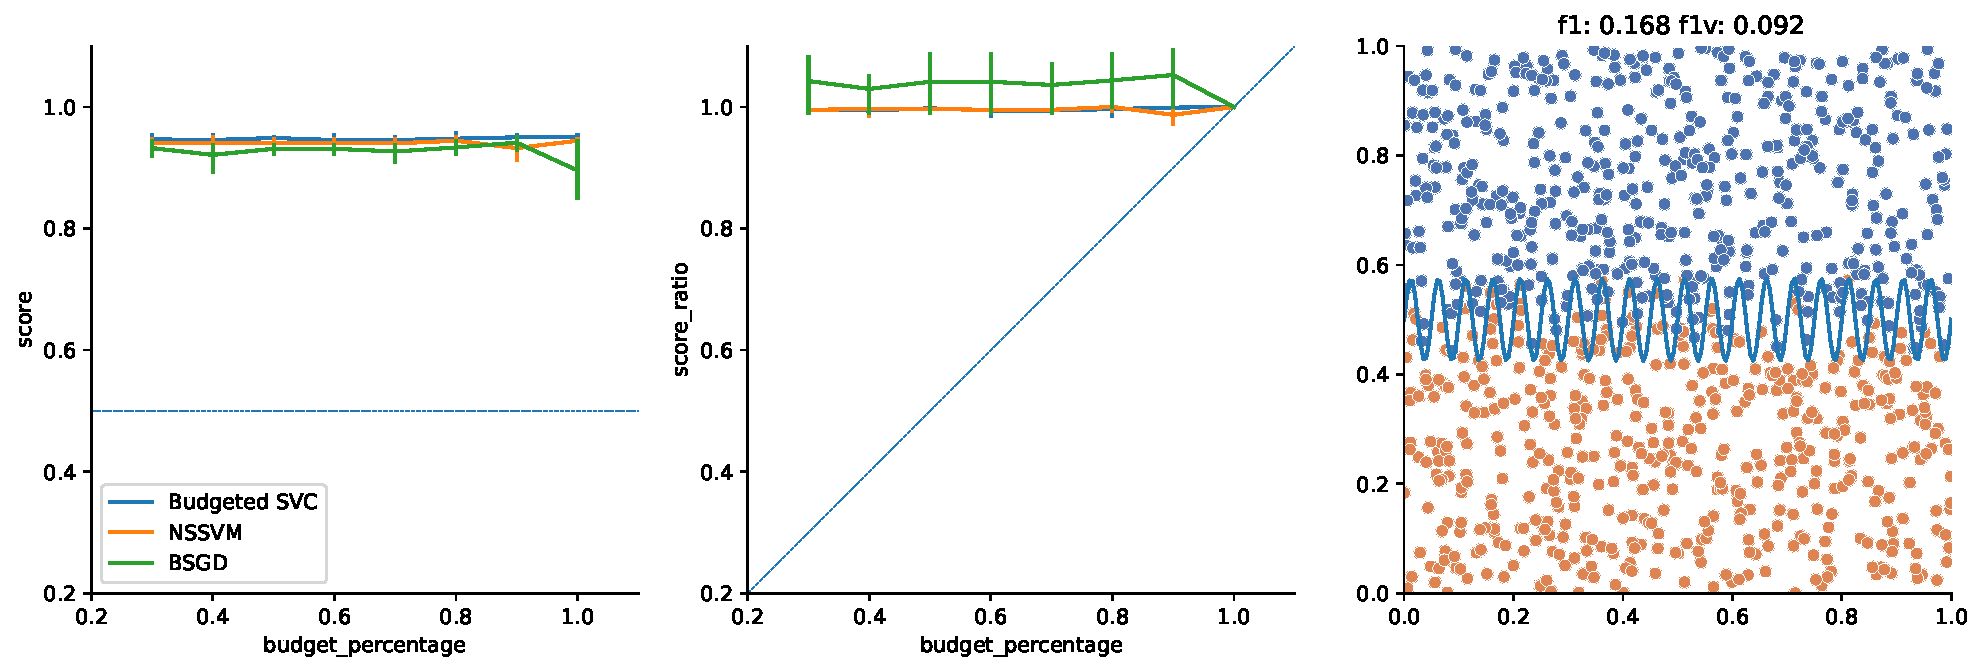
\includegraphics[width=\textwidth]{img/comp_old/9.pdf}
    \end{subfigure}%
    \begin{subfigure}{.5\textwidth}
        \centering
        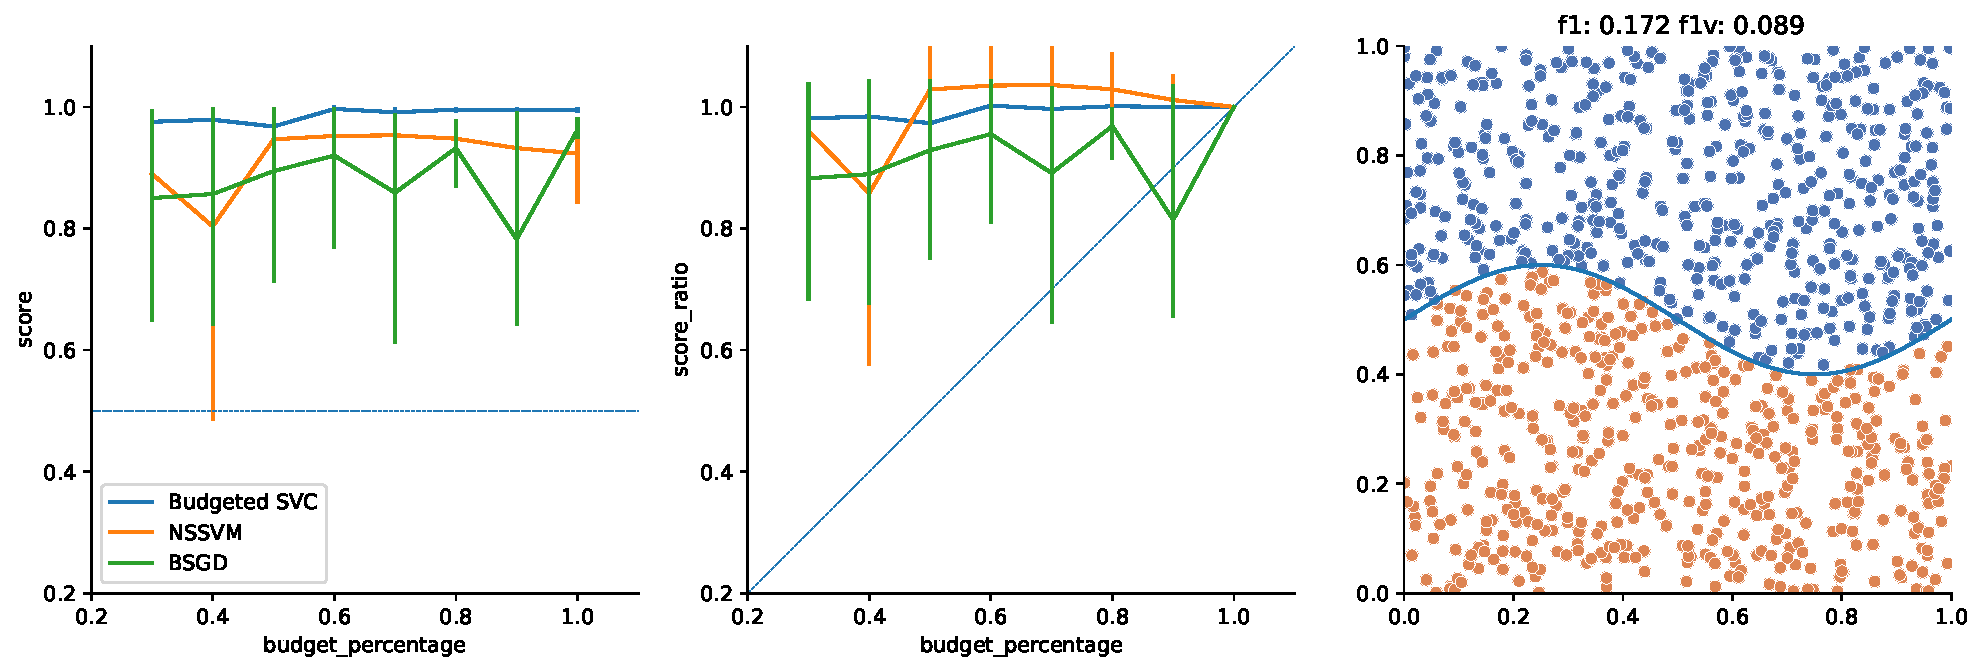
\includegraphics[width=\textwidth]{img/comp_old/10.pdf}
    \end{subfigure}
    %
    \hfill
    %
    \begin{subfigure}{.5\textwidth}
        \centering
        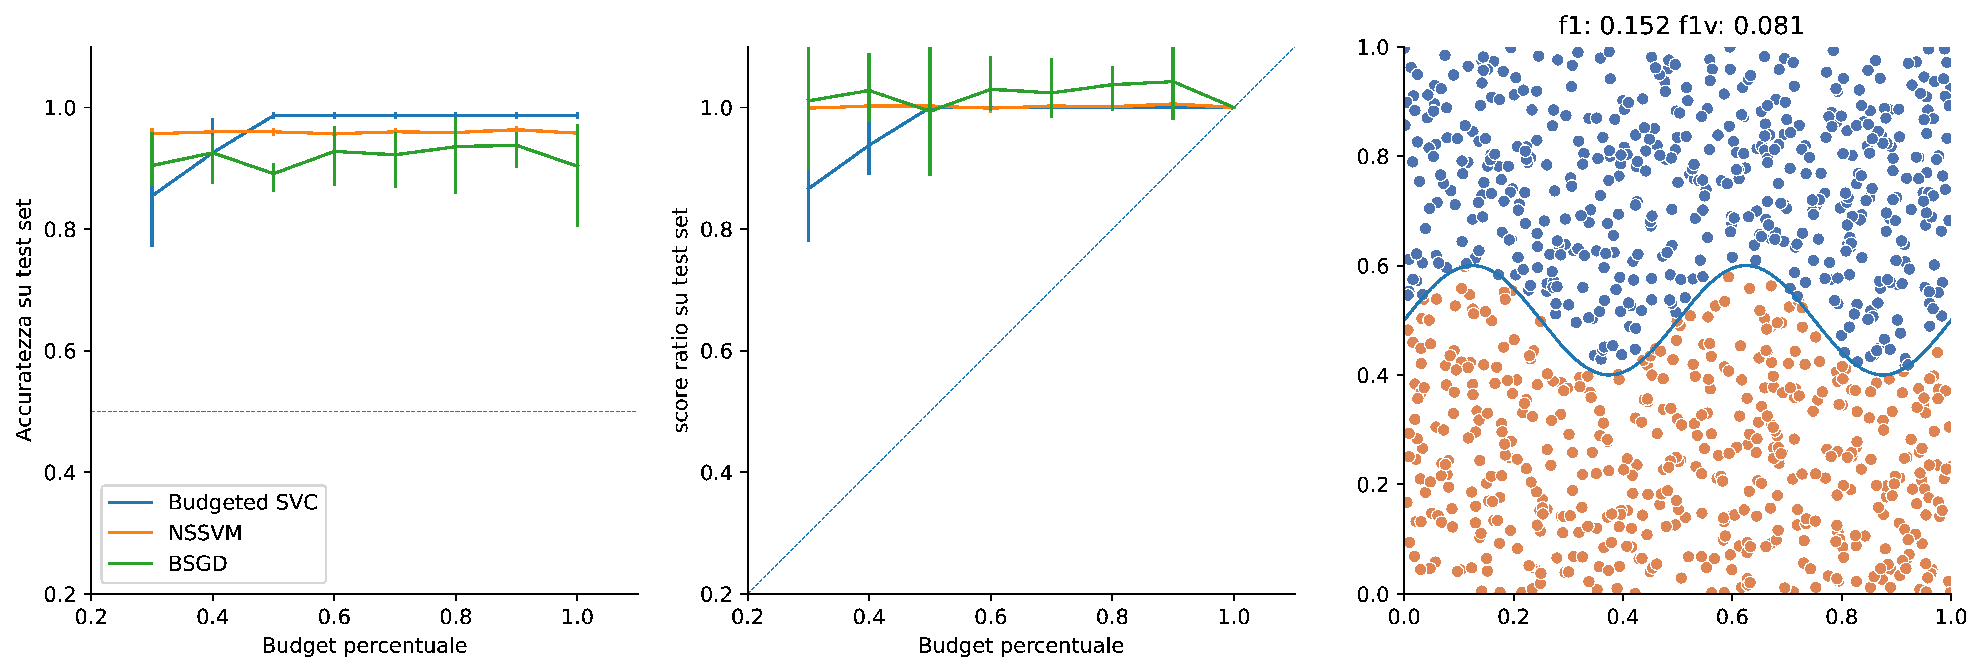
\includegraphics[width=\textwidth]{img/comp_old/11.pdf}
    \end{subfigure}
    \begin{subfigure}{.5\textwidth}
        \centering
        \includegraphics[width=\textwidth]{img/comp_old/12.pdf}
    \end{subfigure}%
    %
    \hfill
    %
    \begin{subfigure}{.5\textwidth}
        \centering
        \includegraphics[width=\textwidth]{img/comp_old/13.pdf}
    \end{subfigure}
    \begin{subfigure}{.5\textwidth}
        \centering
        \includegraphics[width=\textwidth]{img/comp_old/14.pdf}
    \end{subfigure}%
    %
    \hfill
    %
    \begin{subfigure}{.5\textwidth}
        \centering
        \includegraphics[width=\textwidth]{img/comp_old/15.pdf}
    \end{subfigure}
\caption{Esperimenti su dataset sintetici 2D con variazione del budget in funzione della dimensione del dataset, analogo ai risultati in~\Cref{fig:risultati_2d_1,fig:risultati_2d_2} ma con una curva ogni metodo utilizzato: la proposta \emph{Budgeted SVC}, i metodi \emph{NSSVM} e \emph{BSGD}.}
\label{fig:comp_old_2}
\end{figure}   
Nelle~\Cref{fig:comp_new_1,fig:comp_new_2} si possono vedere i valori di accuratezza ottenuti da questi metodi definendo il budget in funzione della dimensione del dataset e confrontati con i risultati ottenuti con \emph{budgeted SVC} e i dataset utilizzati.
\begin{figure}
    \begin{subfigure}{.5\textwidth}
        \centering
        \includegraphics[width=\textwidth]{img/comp_new/1.pdf}
    \end{subfigure}%
    \begin{subfigure}{.5\textwidth}
        \centering
        \includegraphics[width=\textwidth]{img/comp_new/2.pdf}
    \end{subfigure}
    %
    \hfill
    %
    \begin{subfigure}{.5\textwidth}
        \centering
        \includegraphics[width=\textwidth]{img/comp_new/3.pdf}
    \end{subfigure}
    \begin{subfigure}{.5\textwidth}
        \centering
        \includegraphics[width=\textwidth]{img/comp_new/4.pdf}
    \end{subfigure}%
    %
    \hfill
    %
    \begin{subfigure}{.5\textwidth}
        \centering
        \includegraphics[width=\textwidth]{img/comp_new/5.pdf}
    \end{subfigure}
    \begin{subfigure}{.5\textwidth}
        \centering
        \includegraphics[width=\textwidth]{img/comp_new/6.pdf}
    \end{subfigure}%
    %
    \hfill
    %
    \begin{subfigure}{.5\textwidth}
        \centering
        \includegraphics[width=\textwidth]{img/comp_new/7.pdf}
    \end{subfigure}
    \begin{subfigure}{.5\textwidth}
        \centering
        \includegraphics[width=\textwidth]{img/comp_new/8.pdf}
    \end{subfigure}
\caption{Esperimenti su dataset sintetici 2D con variazione del budget in funzione della dimensione del dataset, analogo ai risultati in~\Cref{fig:risultati_2d_1,fig:risultati_2d_2} ma con una curva ogni metodo utilizzato: la proposta \emph{Budgeted SVC}, i metodi \emph{NSSVM} e \emph{BSGD}.}
\label{fig:comp_new_1}
\end{figure}   
\begin{figure}
    \begin{subfigure}{.5\textwidth}
        \centering
        \includegraphics[width=\textwidth]{img/comp_new/9.pdf}
    \end{subfigure}%
    \begin{subfigure}{.5\textwidth}
        \centering
        \includegraphics[width=\textwidth]{img/comp_new/10.pdf}
    \end{subfigure}
    %
    \hfill
    %
    \begin{subfigure}{.5\textwidth}
        \centering
        \includegraphics[width=\textwidth]{img/comp_new/11.pdf}
    \end{subfigure}
    \begin{subfigure}{.5\textwidth}
        \centering
        \includegraphics[width=\textwidth]{img/comp_new/12.pdf}
    \end{subfigure}%
    %
    \hfill
    %
    \begin{subfigure}{.5\textwidth}
        \centering
        \includegraphics[width=\textwidth]{img/comp_new/13.pdf}
    \end{subfigure}
    \begin{subfigure}{.5\textwidth}
        \centering
        \includegraphics[width=\textwidth]{img/comp_new/14.pdf}
    \end{subfigure}%
    %
    \hfill
    %
    \begin{subfigure}{.5\textwidth}
        \centering
        \includegraphics[width=\textwidth]{img/comp_new/15.pdf}
    \end{subfigure}
\caption{Esperimenti su dataset sintetici 2D con variazione del budget in funzione della dimensione del dataset, analogo ai risultati in~\Cref{fig:risultati_2d_1,fig:risultati_2d_2} ma con una curva ogni metodo utilizzato: la proposta \emph{Budgeted SVC}, i metodi \emph{NSSVM} e \emph{BSGD}.}
\label{fig:comp_new_2}
\end{figure}   








